\documentclass[preprint2,numberedappendix,tighten,twocolappendix]{aastex6}  % USE THIS TO MAKE BIB, THEN FORMAT USING EMULATEAPJ
%\documentclass[twocolumn,apj,numberedappendix]{emulateapj}
\shorttitle{Data Analysis Methods for the Detection of the Epoch of Reionization}
\shortauthors{Cheng et al.}

\usepackage{amsmath}
\usepackage{graphicx}
\usepackage[figuresright]{rotating}
\usepackage{natbib}
\usepackage{ctable}
\citestyle{aa}

%		Math Shortcuts from Adrian
%\def\b{\mathbf{b}}
%\def\k{\mathbf{k}}
%\def\r{\mathbf{r}}
%\def\q{\mathbf{q}}
%\def\b{\mathbf{b}}
%\def\kp{\mathbf{k}^\prime}
%\def\kpp{\mathbf{k}^{\prime\prime}}
%\def\V{\mathbb{V}}
%\def\At{\tilde{A}}
%\def\Vt{\tilde{V}}
%\def\Tt{\tilde{T}}
%\def\tb{\langle T_b\rangle}
%\newcommand{\vis}{\mathbf{v}}
%\newcommand{\x}{\mathbf{x}}
%\newcommand{\xhat}{\hat{\mathbf{x}}}
%\newcommand{\nhat}{\hat{\mathbf{n}}}
%\newcommand{\A}{\mathbf{A}}
%\newcommand{\N}{\mathbf{N}}
%\newcommand{\rhat}{\hat{\mathbf{r}}}
%\newcommand{\khat}{\hat{\mathbf{k}}}
%\newcommand{\btheta}{\boldsymbol \theta}

\newcommand{\cc}[1]{{\color{purple} \textbf{[#1]}}}

\begin{document}
\title{Data Analysis Methods for the Detection of the Epoch of Reionization}

\author{
Carina Cheng\altaffilmark{1},
et al.
}


%		Notes	
	
%Reference section with: \ref{sec:Intro}
%Reference equation with: \eqref{eq:eqtest}
%Reference figure with: \ref{fig:figtest}
%Cite paper inside sentence: \citet{ref}
%Cite paper at end of sentence: \citep{ref}
%Cite paper inside a parenthetical sentence: \citealt{ref}

%To compile with references shown, compile in BibTeX once and LaTeX twice


%		Sample Equation Syntax
%\begin{equation}
%\label{eqtest}
%\langle \widetilde{T} (\mathbf{k}) \widetilde{T}^* (\mathbf{k^\prime}) \rangle = (2 \pi)^3 \delta^D (\mathbf{k} - \mathbf{k}^\prime) P(k),
%\end{equation}


\altaffiltext{1}{Astronomy Dept., U. California, Berkeley, CA}
%\altaffiltext{2}{Hubble Fellow}
%\altaffiltext{2}{Radio Astronomy Lab., U. California, Berkeley, CA}
%\altaffiltext{3}{Berkeley Center for Cosmological Physics, Berkeley, CA}
%\altaffiltext{3}{Dept. of Physics and Astronomy, U. Pennsylvania, Philadelphia, PA}
%\altaffiltext{8}{School of Earth and Space Exploration, Arizona State U., Tempe, AZ}

\begin{abstract}
The Epoch of Reionization (EoR) is an uncharted era in our Universe's history during which the birth of the first stars and galaxies led to the ionization of neutral hydrogen. This important epoch of our cosmic dawn harbors a wealth of information regarding the environment during this transformative time, including insight into the nature of the first luminous sources and implications about cosmological parameters. There are many experiments investigating the EoR by tracing the $21$ cm line of neutral hydrogen, a signal which is very faint and difficult to isolate. With a new generation of instruments and a statistical power spectrum detection in our foreseeable future, it has become increasingly important to develop techniques that help maximize sensitivity and validate results. Additionally, it is imperative to understand the trade-offs between different methods and their effects on common power spectrum themes. In this paper, we focus on three major themes - signal loss, power spectrum error bar estimation, and bias in measurements. We describe techniques that affect these themes using both a toy model and data taken by the 64-element configuration of the Donald C. Backer Precision Array for Probing the Epoch of Reionization (PAPER).
\end{abstract}


\section{Introduction}
\label{sec:Intro}

By about one billion years after the Big Bang, the very first stars and galaxies are thought to have ionized all the neutral hydrogen that dominated the baryonic matter content in the early Universe. This transition period, during which the first luminous structures formed from gravitational collapse and began to emit intense radiation that ionized the cold neutral gas into a plasma, is known as the epoch of reionization (EoR). The EoR is a relatively unexplored era in our cosmic dawn. Its history encodes important information regarding the nature of the first galaxies and the processes of structure formation. Direct measurements of the EoR would unlock powerful information about the intergalactic medium, revealing connections between the smooth matter distribution exhibited via cosmic microwave background (CMB) studies and the highly structured web of galaxies we observe today.

One promising technique to probe the EoR is to target the 21 cm wavelength emission that is emitted by neutral hydrogen via its spin-flip transition. This technique is powerful because it can be observed as a function of redshift --- that is, the wavelength of the signal reaching our telescopes can be directly mapped to a distance from where the emission originated before stretching out as it traveled through expanding space. The 21 cm line therefore offers a window into the evolution of ionization, temperature, and density fluctuations on cosmic scales.

Although a detection of the EoR remains elusive, there are several radio telescope experiments that have succeeded in using the 21 cm signal from hydrogen to place constraints on the brightness of the EoR. Examples of experiments investigating the mean brightness temperature of the EoR relative to the CMB are the Experiment to Detect the Global EoR Signature (EDGES, \citealt{bowman2010}), the Long Wavelength Array (LWA, \citealt{ellingson_et_al2009}),  the Large Aperture Experiment to Detect the Dark Ages (LEDA, \citealt{greenhill_bernardi2012}), the Dark Ages Radio Explorer (DARE, \citealt{burns2012}), the Sonda Cosmol\'ogica de las Islas para la Detecci\'on de Hidr\'ogeno NeutroSciHi (SCI-HI, \citealt{voytek2014}), the Broadband Instrument for Global HydrOgen ReioNisation Signal (BIGHORNS, \citealt{sokolowski2015}), and the Shaped Antenna measurement of the background RAdio Spectrum (SARAS, \citealt{patra2015}). Radio interferometers which seek to measure statistical power spectra include the Giant Metre-wave Radio Telescope (GMRT, \citealt{paciga_et_al2013}), the LOw Frequency ARray (LOFAR,\citealt{van_haarlem_et_al2013}), the Murchison Widefield Array (MWA, \citealt{tingay_et_al2013}), the 21 Centimeter Array (21CMA, \citealt{peterson_et_al2004}, \citealt{wu2009}), and PAPER (\citealt{parsons_et_al2010}). The Hydrogen Epoch of Reionization Array (HERA), which is currently being built, is a next-generation instrument that aims to combine lessons learned from previous experiments and is forecasted to be able to make a successful $23\sigma$ detection with an eventual $350$ elements, using current analysis techniques (\citealt{deboer_et_al2017}, \citealt{pober_et_al2014}).

The major challenge that faces all 21 cm experiments is isolating a small signal that is buried underneath foregrounds and instrumental systematics that are 4-5 orders of magnitude brighter. A clean measurement therefore requires an intimate understanding of the instrument and a rigorous study of data analysis choices. With continual progress being made in the field and HERA on the horizon, it is becoming increasingly important to understand how the methods we choose interact with each other to affect power spectrum results. In this paper, we discuss three themes essential to a $21$ cm power spectrum analysis and how data analysis choices affect each. We approach these themes from a broad perspective, and then perform a detailed case study using data from the 64-element configuration of PAPER.

This paper is organized as follows. In section 2 we introduce the three themes of our focus, using a toy model to develop intuition into each one. Section 3 presents an overview of the PAPER-64 array and observations, highlighting key changes from \citet{ali_et_al2015}. Sections 4, 5, and 6 detail how the new PAPER-64 analysis quantifies signal loss, estimates error bars, and eliminates bias, respectively. We conclude in Section 7.

\section{Power Spectrum Themes and Techniques}
\label{sec:Themes}

There are many choices for a data analyst, such as how to combine time-ordered measurements, how to estimate its variance, how to weight data in a way that suppresses contaminated modes while not destroying an EoR signal, and how to identify the source of a detection. Many common techniques, such as averaging data, weighting, bootstrapping, and jack-knife testing, each address these issues yet harbor additional trade-offs. For example, an aggressive filtering method may succeed in eliminating interfering systematics but comes at the cost of losing some EoR signal. A chosen weighting scheme may maximize sensitivity but fail to suppress foregrounds.

Measuring the statistical $21$ cm power spectrum requires robust methods for determining accurate confidence intervals and rigorous techniques to identify and suppress systematics. Additionally, we desire to maximize our sensitivity with filtering and weighting techniques. In this paper, we focus on four techniques and their effects on three overarching themes of $21$ cm power spectrum estimation. We will give brief definitions now, and build intuition for each theme in the sections to follow.

\begin{center}
Power Spectrum Themes
\end{center}
\begin{itemize}
\item[] The accuracy and interpretation of a $21$ cm power spectrum can be encompassed in the following three themes.
\item \textbf{Signal Loss} (Section \ref{sec:SiglossOverview}): As explained in the next section, certain analysis techniques can lead to the loss of the EoR signal. If not corrected for, it could lead to a false non-detection. Computing signal loss has subtle challenges but is crucial to the accuracy of any result.
\item \textbf{Error Bar Estimation} (Section \ref{sec:ErrorOverview}): Confidence intervals on the $21$ cm power spectrum result determine the difference between a detection and a null result, which have two very different implications. Errors can be estimated in a variety of ways, and we will discuss a few of them.
\item \textbf{Bias} (Section \ref{sec:BiasOverview}): There are several possible sources of bias in a visibility measurement that can leak its way into a power spectrum, such as bias from noise and foregrounds. Proving a bias is EoR may be the most difficult challenge for $21$ cm analyses, as it is crucial to be able to distinguish a detection of foreground leakage, for example, from that of EoR. In this paper we will highlight some sources of bias and discuss ways to mitigate its effects.
\end{itemize}

\begin{center}
Power Spectrum Techniques
\end{center}
\begin{itemize}
\item[] The following techniques each have advantages when it comes to maximizing sensitivity and understanding systematics in data. However, they also have limitations and circumstances in which there are trade-offs.
\item \textbf{Fringe-rate filtering:} Fringe-rate filtering can be considered an averaging scheme for time-ordered data (\citealt{parsons_et_al2016}), and we explain the trade-offs of filtering in more detail in Section \ref{sec:SiglossOverview}. Broadly, a fringe-rate filter increases the sensitivity of a dataset and reduces the number of independent samples by an amount dependent on the width of the averaging window. However, it can also affect the presence of foregrounds and systematics. 
\item \textbf{Weighting:} A dataset can be weighted to emphasize certain spectral features and minimize others. One particular flavor of weighting is inverse covariance weighting, which weights a dataset by minimizing the covariance between frequency channels. This weighting has the effect of down-weighting correlated information (i.e. foregrounds) and up-weighting noise-like information (i.e. EoR). However, one challenge of weighting is in accurately determining a covariance matrix that best describes the data.
\item \textbf{Bootstrapping:} Because applying theoretical errors to a $21$ cm measurement are insufficient \cc{why?}, bootstrapping is a useful method for estimating errors of a dataset from itself. By randomly drawing many samples of the data, we get a sense of its inherent variance, though there are subtleties to consider such as bootstrapping sample sizes.
\item \textbf{Jack-Knife testing:} A resampling technique useful for estimating bias, jack-knives can be taken along different dimensions of a dataset to cross-validate results. In particular, null tests can be used to verify whether results are free of systematics (\citealt{keating_et_al2016}).
\end{itemize}

In the next three subsections, we go into each theme in depth, focusing on how power spectrum technique trade-offs affect each. We use a toy data model to develop intuition into why certain analysis choices may be appealing and discuss ways in which they are limited. We highlight problems that can arise regarding each theme and offer suggestions to mitigate the issues. Ultimately, \cc{some kind of summarizing sentence here}.

\subsection{Signal Loss}
\label{sec:SiglossOverview}

Signal loss refers to the attenuation of the target cosmological signal in a dataset. It can arise in a variety of ways in the analysis pipeline, such as fitting a polynomial during spectral calibration, applying a delay-domain filter, or by weighting data by itself. Here we focus on signal loss associated with applying a weighting matrix to data. Driven by the need to mitigate foreground bias, we would like to use a weighting method that succeeds in down-weighting foregrounds. However, as we'll investigate, this carries the risk of large amounts of signal loss. 

Before we demonstrate how different weighting matrices affect signal loss, we first recap how weights are related to the power spectrum estimation technique of optimal quadratic estimators (OQE, \citealt{liu_et_al2014b}). A summary of the method is as follows. 

We begin with our data vector, $\textbf{x}$, which contains our measured visibilities in mK that have the shape ($times$, $frequencies$). We form the un-normalized power spectrum estimate $\hat{q}_{\alpha}$:

\begin{equation}
\label{eq:qhat}
\hat{q}_{\alpha} = \frac{1}{2}\textbf{x}^{\dagger}\textbf{w}\textbf{Q}_{\alpha}\textbf{w}\textbf{x}
\end{equation}

where $\textbf{w}$ \cc{change to capital letter that isn't taken yet!} is a weighting matrix (for example, inverse covariance weighting would set $\textbf{w} = \textbf{C}^{-1}$). The matrix $\textbf{Q}$ is an operator that takes our frequency-domain visibilities and Fourier-transforms them into power spectrum space. The index $\alpha$ denotes a waveband in $k_{\parallel}$, where $k_{\parallel}$ is the Fourier-dual to frequency.

We normalize our power spectrum estimates using the matrix $\textbf{M}$:

\begin{equation}
\hat{\textbf{p}} = \textbf{M}\hat{\textbf{q}}
\end{equation}

where $\hat{\textbf{p}}$ is the normalized estimate of the true power spectrum . We compute $\textbf{M}$ using the Fisher matrix $\textbf{F}$, defined as:

\begin{eqnarray}
\textbf{F}_{\alpha\beta} &=& \frac{1}{2}tr[\textbf{w}\textbf{Q}_{\alpha}\textbf{w}\textbf{Q}_{\beta}]. 
\end{eqnarray}

We have a choice for $\textbf{M}$, and for simplicity in this section we set $\textbf{M} \propto \textbf{I}$, the identity matrix. This is not the case for the analysis of PAPER-64 data, which we describe in Section \cc{not sure which section to point to yet} as part of the discussion of bias. 

In the next sections, we will experiment with different weighting matrices $\textbf{w}$ and their impact on the resulting power spectra estimate $\hat{\textbf{p}}$.

\subsubsection{Toy Model: Inverse Covariance Weighting}

To build our intuition into how a particular choice of weighting, namely inverse covariance weighting, can lead to signal loss through the use of a toy model. Suppose we have a very simple dataset that contains 2-dimensional data (representing $100$ time integrations and $20$ frequency channels). This model represents realistic dimensions of about an hour of PAPER data which could be used for a power spectrum analysis. We create a mock bright foreground signal, $\textbf{x}_{FG}$, as a complex sinusoid that varies in time and frequency, as well as a mock EoR signal, $\textbf{x}_{EoR}$, as complex, random Gaussian noise. The sum of the two forms our combined data vector, $\textbf{x}$, to which we will be applying different weighting schemes. The three data vectors are shown on in Figure \ref{fig:toy_sigloss1}. Our ultimate goal in experimenting with weighting is to suppress the foregrounds perfectly without destroying EoR.

One choice for a weight matrix $\textbf{w}$ is an inverse covariance matrix. This type of weighting is attractive for power spectrum analyses because it is an aggressive way to down-weight foregrounds. The covariance matrix $\textbf{C}$, which describes covariances between frequency channels, can be estimated in a variety of ways. Should we have perfect foreground, instrumental, and EoR models, we could form $\textbf{C}$ in a way that accurately describes our real data. However, if our foreground model is flawed for example, our estimate of $\textbf{C}$ would not be successful at down-weighting the real foregrounds in the data. One attractive way to estimate $\textbf{C}$ then is to empirically derive it from the data vector $\textbf{x}$ itself:

\begin{equation}
\textbf{C} \equiv \langle\textbf{xx}^{\dagger}\rangle,
\end{equation}

assuming $\langle\textbf{x}\rangle = 0$. The inverse covariance matrix is therefore $\textbf{w} = \textbf{C}^{-1}$.

If $\textbf{C}$ is computed from the data itself and its inverse is then applied to the data, it carries the risk of over-fitting information in the data and introducing a multiplicative bias to estimates of the signal. If instead we choose $\textbf{w} = \textbf{I}$, the identity matrix, there will be no signal loss (although it may suffer from foreground or instrumental bias). We will refer to this choice as `unweighted', since using the identity does not alter (doesn't upweight or downweight) the data at all.

\begin{figure}
	\centering
	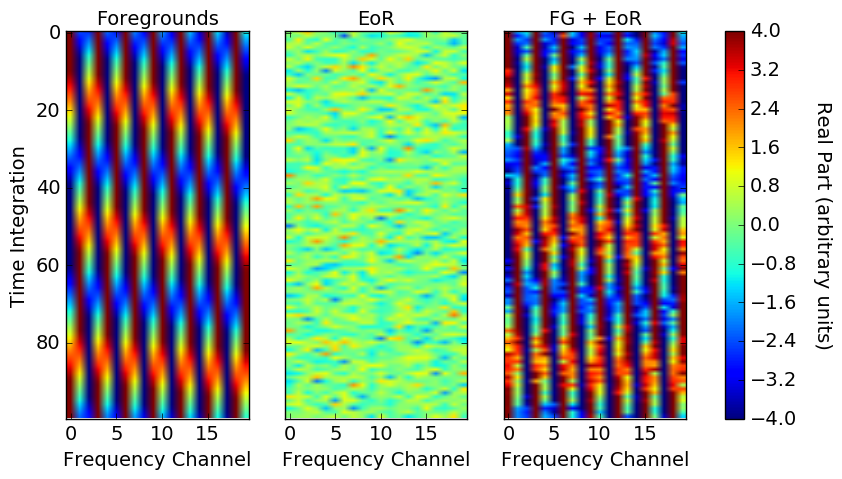
\includegraphics[trim={0.3cm 0.2cm 0.3cm 0.3cm},clip,width=\columnwidth]{plots/toy_sigloss1.png}
	\caption{Our toy model dataset contains a sinusoid foreground that varies in time and frequency and random Gaussian noise as a mock EoR signal. Real parts are shown here.}
	\label{fig:toy_sigloss1}
\end{figure}

First, we compute the power spectrum of $\textbf{x}$ using the OQE formalism and a weighting matrix of $\textbf{C}^{-1}$. The result is shown in green in the left plot of Figure \ref{fig:toy_sigloss3}. Also plotted in the figure are the unweighted power spectrum of $\textbf{x}_{FG}$ (blue) and $\textbf{x}_{EoR}$ (red). 

\begin{figure*}
	\centering
	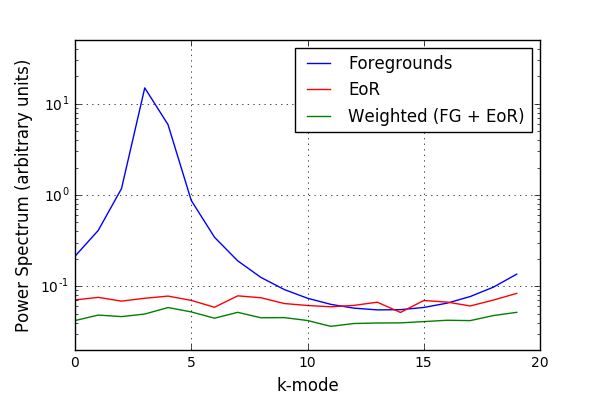
\includegraphics[trim={0.3cm 0.2cm 1cm 0.3cm},clip,height=0.3\textwidth]{plots/toy_sigloss3.png}
	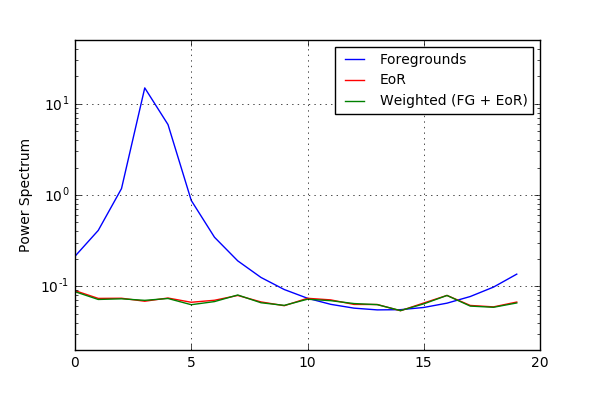
\includegraphics[trim={1cm 0.2cm 0cm 0.3cm},clip,height=0.3\textwidth]{plots/toy_sigloss4.png}
	\caption{Power spectrum of foregrounds only (blue), EoR only (red), and the combined dataset (green). Contrasted are the effect of using inverse covariance weighting (left) and projecting out the first eigenmode only (right).}
	\label{fig:toy_sigloss3}
\end{figure*}

As shown in Figure \ref{fig:toy_sigloss3}, our inverse covariance weighted result successfully suppresses foregrounds. This illustrates why inverse covariance weighting is attractive for $21$ cm data. It is also evident that our result fails to recover the EoR signal --- it exhibits the correct shape, but the amplitude level is slightly low. This is evidence of signal loss. In order to understand how this occurs, we need to closely study our covariance matrix, $\textbf{C}$.

It turns out that because we estimated $\textbf{C}$ from our data, its eigenspectrum offers insight into understanding how inverse covariance weighting affects our result. An eigenspectrum ranks the eigenvalues of $\textbf{C}$ from highest to lowest and can be thought of as a spectrum of weights that are given to each frequency mode in the data. The eigenspectrum of the identity matrix $\textbf{I}$ is flat (all $1$'s) because it gives equal weighting to all modes. 

\begin{figure}
	\centering
	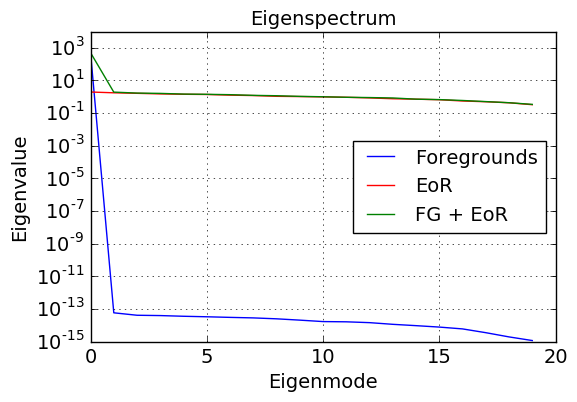
\includegraphics[trim={0.3cm 0.2cm 0.3cm 0.3cm},clip,width=\columnwidth]{plots/toy_sigloss2.png}
	\caption{Eigenspectrum of foregrounds only (blue), EoR only (red), and FG + EoR (green).}
	\label{fig:toy_sigloss2}
\end{figure}

For our toy model, the eigenspectra of $\textbf{C}_{FG}$, $\textbf{C}_{EoR}$, and $\textbf{C}$ are shown in Figure \ref{fig:toy_sigloss2}. The blue curve peaks only at the zeroth eigenmode, revealing that the foregrounds can be described by a single eigenmode. This is a direct consequence of how it was constructed (only one sinusoid). In fact, the blue peak in Figure \ref{fig:toy_sigloss3} is also a direct result of our foreground's construction. The eigenspectrum of EoR, however, is fairly flat, signifying that its covariance matrix is similar to an identity matrix. This makes sense because the EoR signal consists of random noise, which should only have strong frequency-frequency correlations when two frequencies are the same.

The eigenmodes with the highest eigenvalues will be down-weighted the most (i.e. when the spectrum is inverted, they will be given the smallest weights). In contrast, the modes with the smallest eigenvalues will be up-weighted the most. In other words, if an eigenspectrum is not perfectly flat, all modes will be given different weights and it is possible to up-weight a few modes much more than others. The subtle slope of the eigenspectrum in this toy example gives rise to a small amount of signal loss because it is possible to overfit a few modes (the highest weighted ones) ever so slightly. We will see in the next section how this effect can be exaggerated as the `steepness' of the spectrum changes.

Using what we've learned about the eigenspectrum, we can tweak it in a simple way to suppress foregrounds and yield zero signal loss. Namely, we can zero out all eigenmodes except the first one, thereby down-weighting the foregrounds perfectly and nothing else. The result is shown in the right plot of Figure \ref{fig:toy_sigloss3}. In this case, we perfectly recover EoR, demonstrating that if we can perfectly model our foregrounds, we can down-weight them without signal loss. However, this is not the case in reality since we aren't able to distinguish between foreground and EoR modes.

\subsubsection{Toy Model: Fringe-Rate Filtering}

We have shown how signal loss can arise due to unintentionally up-weighting eigenmodes with small eigenvalues (overfitting the noise). We will next show how this effect is exaggerated with a reduction of the total number of independent samples in a dataset. 

A fringe-rate filter is an analysis technique designed to maximize sensitivity by integrating in time (\citealt{parsons_et_al2016}). To mimic this filter, we average every $4$ time integrations of our toy model dataset together, yielding $25$ independent samples in time (Figure \ref{fig:toy_sigloss5}, left). We choose these numbers so that the total number of independent samples is similar to the number of frequency channels (our matrices will be full rank). The resulting eigenspectra (Figure \ref{fig:toy_sigloss5}, right), as compared to those in Figure \ref{fig:toy_sigloss1}, fall more steeply for last few eigenmodes. This shape has large consequences on the resulting power spectra.

\begin{figure*}
	\centering
	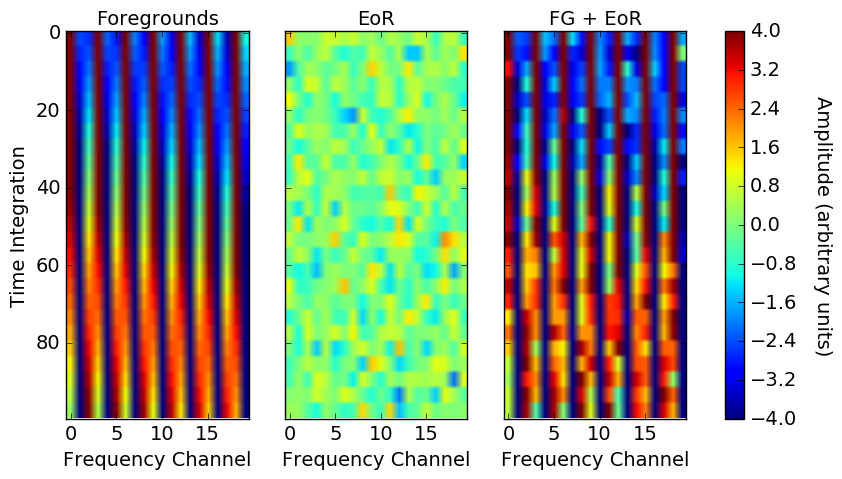
\includegraphics[trim={0.3cm 0.2cm 0.3cm 0.3cm},clip,height=0.3\textwidth]{plots/toy_sigloss5.png}
	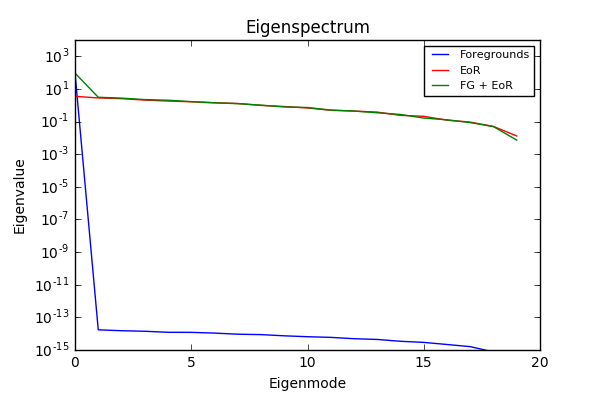
\includegraphics[trim={0.3cm 0.2cm 0.3cm 0.3cm},clip,height=0.3\textwidth]{plots/toy_sigloss6.png}
	\caption{Left: Our `fringe-rate filtered' toy model dataset. It contains $25$ independent samples in time. Real parts are shown here. Right: Eigenspectrum of foregrounds only (blue), EoR only (red), and both (green).}
	\label{fig:toy_sigloss5}
\end{figure*}

\begin{figure}
	\centering
	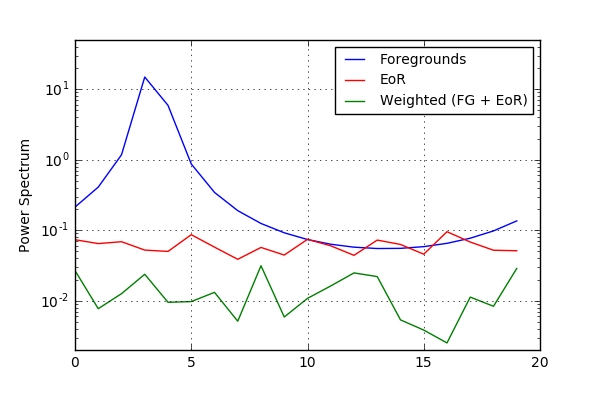
\includegraphics[trim={0.3cm 0.3cm 0.3cm 0.3cm},clip,width=\columnwidth]{plots/toy_sigloss7.png}
	\caption{Power spectrum of foregrounds only (blue), EoR only (red), and the full inverse covariance weighted combined dataset (green) for a time-averaged dataset (fewer independent modes).}
	\label{fig:toy_sigloss7}
\end{figure}

Applying inverse covariance weighting to this dataset results in the power spectra shown in Figure \ref{fig:toy_sigloss7}. There is a much larger amount of signal loss for this time-averaged dataset. To reiterate, the drop-off in the eigenspectrum shape suggests that when the spectrum is inverted, a few modes are up-weighted much more strongly than the rest. This dramatic up-weighting drowns out the EoR signal, giving rise to signal loss. Additionally, most of our power spectrum information is coming from only the last few modes and as a result, is a noisier estimate. This is evident by noticing that the green curve in Figure \ref{fig:toy_sigloss7} fails to trace the shape of the unweighted EoR power spectrum.

Using our toy model, we have seen that a sensitivity driven analysis technique like fringe-rate filtering has trade-offs of signal loss and noisier estimates. Longer integrations increase sensitivity but reduce the number of independent samples, resulting in steep drop-offs in eigenspectra. For PAPER-64 data, we see $\sim3$ orders of magnitude of signal loss when combining the use of an optimal fringe-rate filter and inverse covariance weighting. 

\subsubsection{Toy Model: Other Weighting}

In a previous section we showed how altering an eigenspectrum can make the difference between zero and some signal loss, if we can distinguish between foreground eigenmodes and EoR eigenmodes. We will now use our toy model to describe several other ways to alter a covariance matrix $\textbf{C}$ in order to minimize signal loss. 

As a first test, we know that our simulated EoR should have a covariance matrix that mimics the identity matrix, with its variance encoded along the diagonal. If we model $\textbf{C}_{EoR}$ as such, instead of computing it based on the dataset itself, and add it to $\textbf{C}_{FG} = \textbf{x}_{FG}\textbf{x}_{FG}^{\dagger}$ to obtain a final $\textbf{C}$ to use in weighting, we see that there is negligible signal loss (Figure \ref{fig:toy_sigloss8}, upper left).

\begin{figure*}
	\centering
	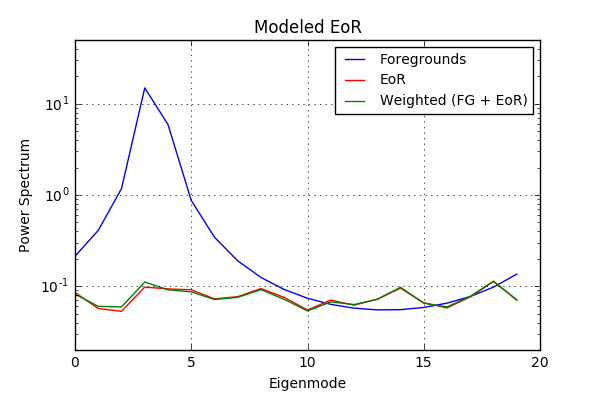
\includegraphics[trim={0.4cm 0.8cm 1.3cm 1cm},clip,height=0.25\textwidth]{plots/toy_sigloss10.png}
	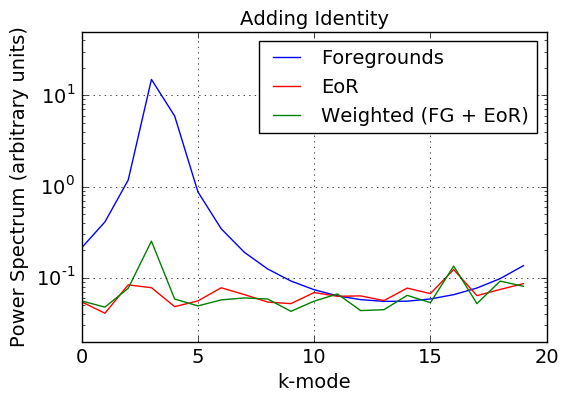
\includegraphics[trim={1cm 0.8cm 1.3cm 1cm},clip,height=0.25\textwidth]{plots/toy_sigloss8.png}
	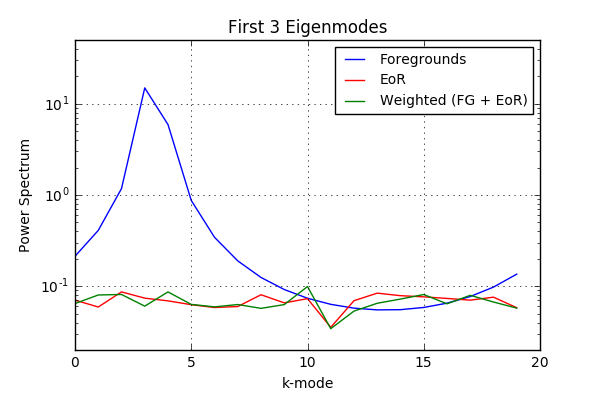
\includegraphics[trim={0.4cm 0.8cm 1.3cm 1cm},clip,height=0.25\textwidth]{plots/toy_sigloss9.png}
	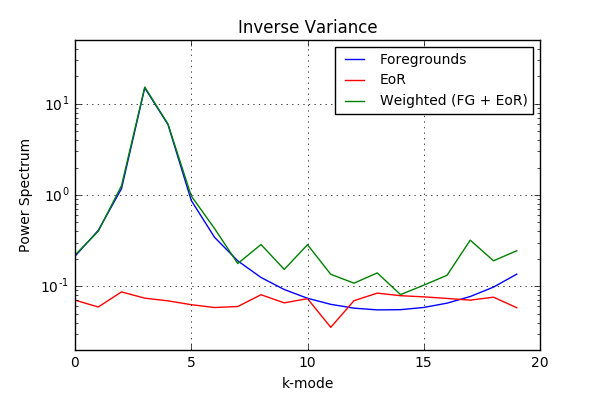
\includegraphics[trim={1cm 0.8cm 1.3cm 1cm},clip,height=0.25\textwidth]{plots/toy_sigloss11.png}
	\caption{Power spectra of foregrounds only (blue), EoR only (red), and the weighted combined dataset (green). We show four alternate weighting options that each avoid signal loss, including modeling the covariance matrix of EoR (upper left), regularizing $\textbf{C}$ by adding an identity matrix to it (upper right), using only the first few eigenmodes of $\textbf{C}$ (lower left), and multiplying an identity matrix to $\textbf{C}$ (lower right).}
	\label{fig:toy_sigloss8}
\end{figure*}

The next three panels of Figure \ref{fig:toy_sigloss8} each involve methods that regularize the matrix $\textbf{C}$ after it is computed from the foreground + EoR dataset. By regularizing $\textbf{C}$, we are flattening out its eigenspectrum. Therefore, some modes will be down-weighted, but the rest will be treated with similar weights. Hence, we won't be up-weighting the last few noisy modes. 

Regularization schemes that we are highlighting here are adding an identity matrix to $\textbf{C}$ (Figure \ref{fig:toy_sigloss8}, upper right), killing all but the first three eigenmodes of $\textbf{C}$ (lower left), and multiplying an identity matrix to $\textbf{C}$ (lower right). Each avoids signal loss, but it is clear that two of the methods down-weight foregrounds much better than the third. For this toy model, our foregrounds are spread out in frequency and therefore have non-negligible frequency-frequency correlations. Therefore, when multiplying $\textbf{C}$ by an identity matrix, we are only preserving correlations between the same frequencies. Because we killed off information from all other frequency combinations, we do a poor job suppressing the foreground.  

Although this method did not successfully recover EoR for this particular simulation, it is important that we show that there are many options for estimating a covariance matrix, and some may work better than others based on the dataset. One may imagine a situation where a particular systematic is contained to an isolated frequency. In such a case, preserving only the diagonal elements of $\textbf{C}$ would be an effective way of removing this contamination. 

In summary, we have a choice of how to weight $21$ cm data. Ideally, we want to down-weight bright foregrounds without removing the underlying cosmological signal. Inverse covariance weighting is an optimal weighting for dealing with foregrounds, but its aggressiveness results in sloped eigenspectra shapes, the overfitting of noise, and thus signal loss. The application of a fringe-rate filter heightens this effect by reducing the number of independent samples and steepening eigenspectra further. Rather than use inverse covariance weighting, there are several alternate ways to regularize covariance matrices and flatten out eigenspectra to minimize signal loss. In Section \ref{sec:Sigloss}, we apply the lessons we've learned about signal loss and its interaction with fringe-rate filtering and inverse covariance weighting to PAPER-64 data.

\subsection{Error Estimation}
\label{sec:ErrorOverview}

Two ways of estimating errors on a power spectrum measurement are exploring the variance of a dataset, and computing a theoretical error estimate based on an instrument's system temperature and observational parameters. In a perfect world, both methods would match up. However, in practice the two don't always agree due to contaminates in the data that prevent it from being perfectly noise-limited. Therefore, it is important to place error bars on our measurements that have been derived from its inherent variance.

A common technique used to estimate the variance in a dataset is bootstrapping. Bootstrapping is a metric that relies on sampling with replacement and allows the estimation of a sampling distribution. For example, power spectrum measurements of $21$ cm data can be made along many axes, including time and baselines. Through the process of bootstrapping, we can obtain error bars for our results which represent the underlying distribution of power spectra values that are allowed by our measurements.

Again, we focus on simple toy models to highlight two traps that one can fall into when bootstrapping power spectra. Suppose we have a Gaussian random noise dataset of length $1000$ and variance of $1$. We are interested in the average of the dataset, and therefore predict that the error on the mean should obey $1/\sqrt{N}$, where $N$ is the number of samples (in this case, $1000$). 

We form $100$ bootstraps, each comprised of an array of length $1000$ that is created by random sampling the original data with replacement. The standard deviation over the $100$ bootstraps gives an error estimation for our dataset. As shown in Figure \ref{fig:toy_error1} (grey star), the error computed from bootstrapping matches our theoretical prediction.

One major caveat of bootstrapping is that the method is no longer valid when working with correlated data. In other words, bootstrapping assumes completely independent samples. Therefore, the use of a fringe-rate filter, which averages data in time to increase sensitivity, creates a situation in which bootstrapping can under-estimate errors.

Going back to our toy model, we apply a sliding boxcar average to $10$ samples at a time, thus reducing the number of independent samples to $1000/10 = 100$. Bootstrapping this time-averaged noise, using the same exact method as described earlier (drawing the same number of samples as the length of the dataset), under-estimates the error by a factor of $\sim3$. This occurs because we are drawing more samples than independent ones available. In fact, the error derived from bootstrapping is a strong function of the number of samples that are drawn (Figure \ref{fig:toy_error1}, black points), and we can both under-estimate the error by drawing too many or over-estimate it by drawing too few. However, in this case we know that we have $100$ independent samples, and the error associated with drawing $100$ samples with replacement does match the theoretical prediction as expected.

This examples highlights the importance of understanding how analysis techniques (like a fringe-rate filter) can affect a common statistical procedure (like bootstrapping). Bootstrapping as a means of estimating power spectrum errors from real fringe-rate filtered data requires precise knowledge of the number of independent samples, which is not a trivial task.

\begin{figure}
	\centering
	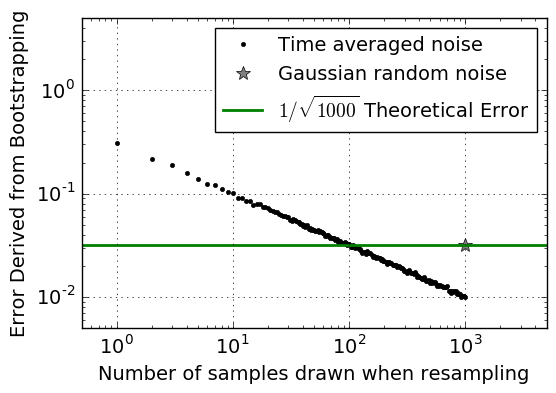
\includegraphics[trim={0.3cm 0.3cm 0.3cm 0.3cm},width=\columnwidth]{plots/toy_error1.png}
	\caption{Error estimation produced by bootstrapping as a function of the number of samples drawn when sampling with replacement. The grey star represents the error associated with drawing $1000$ samples from a length $1000$ array of random noise. The black points correspond to time-averaged data and illustrate how errors can be underestimated if drawing more samples than independent ones in the data. There are $100$ independent samples in the time-averaged data and using this number does indeed match the theoretical error prediction.}
	\label{fig:toy_error1}
\end{figure}

We will now discuss a second subtle feature of bootstrapping that can lead to an over-estimation of errors. Suppose we have $1000$ baselines (another appropriate axis for bootstrapping power spectra), each an independent measurement of the sky. Bootstrap theory requires a bootstrap to comprise of some combination of the $1000$ baselines. If all $1000$ spaces are filled randomly, there is in fact a high probability that baselines will be repeated in a sample (sometimes many times). Thus, bootstrapping in this way negatively affects power spectrum sensitivity because the number of independent baselines in a sample can be significantly lower than the total number of baselines.

In order to maximize sensitivity, we use a slightly modified bootstrapping method. We first shuffle all the baselines for a bootstrap, take the first $999$, and then fill the last slot randomly with replacement. There's a small chance it will yield $1000$ independent samples, but even with $999$ our sensitivity is nearly maximized. One may wonder whether this change is still a legitimate way of error estimating since the number of possible random samples for a single bootstrap has dramatically decreased. However, as long as this number is still much greater than the number of bootstraps we perform, it is a valid way to uncover the inherent variability in a dataset. 

For our toy model, the fraction of independent baselines using this method ($999/1000$) is over $1.5$ times greater than the aforementioned approach. These two methods converge for small numbers of samples, when filling a few spots randomly is nearly the same as filling only the last spot randomly. The evolution of both of these methods as a function of number of baselines is shown in Figure \ref{fig:toy_error2}. In order to reduce the number of baselines, we divide our $1000$ baselines into $N$ groups, where the number of baselines in a group is $1000/N$. No baselines are repeated within or between groups, until a bootstrapping method is applied to each (either sampling all elements with replacement, or only the last one).

It is clear that the fraction of independent baselines in a group is always greater using our new sampling approach, with the greatest discrepancy for small number of groups (large number of baselines per group). An analog for the y-axis in Figure \ref{fig:toy_error2} is the final power spectrum sensitivity in temperature-squared space, which decreases as the square root of the number of baselines that are averaged together for a measurement.

In summary, bootstrapping is still an effective and straightforward way to estimate errors of a dataset. However, one must be careful about violating independence assumptions, as it is possible to under-estimate errors by over-sampling data. Additionally, small changes in the way datasets are randomly sampled can ensure that the overall sensitivity is maximized.

\begin{figure}
	\centering
	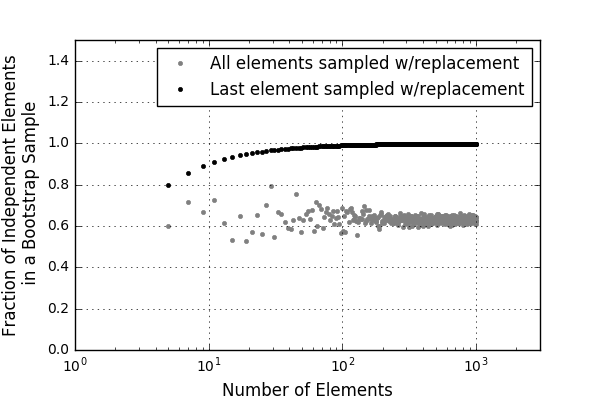
\includegraphics[trim={0.3cm 0.3cm 0.3cm 0.3cm},width=\columnwidth]{plots/toy_error2.png}
	\caption{Fraction of independent baselines in a baseline group as a function of the number of baselines in a group. A fraction of $1.0$ means that all baselines in a group are independent, and therefore sensitivity is maximized (alternatively, this axis can be treated as a power spectrum sensitivity in temperature-squared space). Two bootstrapping methods are shown here --- sampling all elements with replacement (grey) and sampling only the last element with replacement (black). The former over-estimates error bars by not maximizing baseline sensitivity to its full capacity.}
	\label{fig:toy_error2}
\end{figure}

We have discussed the interplay between two of our power spectrum techniques --- fringe-rate filtering and bootstrapping --- and how they affect the theme of error bar estimation. In addition to these, inverse covariance weighting can also affect error bars. Specifically, a power spectrum measurement and its errors are susceptible to blowing up when the number of non-zero eigenmodes are less than the number of independent samples in a dataset (i.e. the covariance matrix is not full rank). \cc{Not really sure how to explain this or how much detail to get into here...}

Our fourth power spectrum technique, jack-knife testing, is also related to error estimation. Splitting data along various axes and performing the same power spectrum analysis on each provides a test of robustness. If the same errors are obtained for each data subset, we can have confidence that they are unbiased.

\subsection{Bias}
\label{sec:BiasOverview}

There are several sources of bias that could leak into a power spectrum measurement, including noise and foreground biases. In this section we will describe analysis techniques that help mitigate these effects and how jack-knife tests can tease out biases that are present in data. Ultimately, while different weighting and data combination techniques can help identify and remove biases, it is important to remember that a true detection of EoR will be robust to these tests. In other words, detections that aren't stable across multiple jack-knives are likely false ones and attributable to systematic errors.

Noise bias can arise in multiple ways. Every $21$ cm visibility measurement contains thermal noise that is comprised of receiver and sky noise. We expect this noise to be independent between antennas and thus we can beat it down (increase sensitivity) by integrating longer, using more baselines, etc. However, a noise bias can result if the same thermal noise is multiplied by itself. This squaring of noise occurs when cross-multiplying visibilities to enter temperature squared space and results in power spectrum measurements that are higher than those predicted by the thermal noise of the instrument. One way to avoid this type of noise bias is to avoid cross-multiplying data from the same baselines or days. This ensures that the two quantities that go into a measurement have separate noises that don't correlate with each other. 

Another way of introducing a noise bias into data is via cross-talk subtraction. Cross-talk is caused by the cross-coupling of signals between antennas and shows up as a constant bias in time in visibilities. For PAPER-64, cross-talk is removed during redundant calibration, when the deviation from an average visibility (across similar baseline types) is subtracted off of each visibility. This type of removal preserves signals common to all baselines, such as the EoR signal, but also has the consequence of introducing a low level bias. This bias term comes from the averaged cross-talk across a redundant baseline group and hence every baseline now has a piece of all the other baseline's (of the same type) noise. One way to remove this noise bias is with the use of a fringe-rate filter, which can be chosen to filter out static signals (filter out zero `fringe-rates').

Foreground bias is perhaps one of the main limiting factors pushing up against $21$ cm results. Foreground signals lie $\sim4-5$ orders of magnitude above the cosmological signal, and there are many existing techniques to avoid or remove these strong signals. Despite current best efforts to do so, however, there remains some foreground leakage that can show up as detections in a power spectrum. This leakage is strongest at low $k$ values, corresponding to large spatial scales on the sky. 

As with noise bias, there are analysis techniques to mitigate the effects of foreground leakage and prevent information from low $k's$ from spreading to high $k$ values. Narrow window functions can be used to minimize the influence of a particular $k$ value on other ones (\cc{citation?}). This in turn compromises power spectrum sensitivity (narrow window functions increases errors for each $k$-mode) as a trade-off for the minimization of foreground leakage. Another option is to construct an estimator using OQE that forces a window function to have a minimum response to low $k$ values. The PAPER-64 window function is constructed in such a way, specifically to prevent foregrounds that live at low $k's$ from contaminating higher $k$-modes (Section \ref{sec:PS}).

One last source of foreground bias that we will highlight here is polarization leakage. When forming Stokes I from $XX$ and $YY$ polarization visibility data, we ignore the beam asymmetry between the two. This mismatch can cause leakage from Stokes Q ($V_{Q} = \frac{1}{2}(V_{XX}-V_{YY})$) into Stokes I ($V_{I} = \frac{1}{2}(V_{XX}+V_{YY})$). Another way of describing this leakage is that Faraday Rotation, which causes a rotation of the polarization angle of a signal, can induce spectral structure at certain delays (\citealt{moore_et_al2013}). This type of sky bias is dependent on rotation measures, which characterize the amount of polarization rotation. If a particular rotation measure is such that a Stokes Q signal ends up falling at a power spectrum delay of interest, the Stokes I result would be biased. 

One preventative measure for polarization leakage could be tailoring a fringe-rate filter in a way that improves the match between $XX$ and $YY$ polarization beams (\citealt{parsons_et_al2016}). There are also multiple ways of tracing a power spectrum detection to a polarization bias. One can look at Stokes Q power spectra to estimate the amount of expected leakage (\citealt{moore_et_al2013}). In addition, jack-knife tests can be used to investigate whether polarization leakage affects a result. For example, rotation measures are highest when observing into the Galactic plane due to increased Faraday rotation (\cc{citation?}), so one could imagine looking at different rotation measure bins along the Galactic latitude axis in order to identify whether a strong rotation measure coincides with a particular power spectrum detection. 

In general, jack-knife tests are helpful in revealing a range of biases, including polarization and foreground biases. Slicing data along LST, for example, can determine whether excess detections are traceable to certain foreground sources. Slicing along baselines can uncover poorly operating baselines, or baselines whose weighting matrices aren't properly down-weighting foregrounds. Jack-knives can be taken along polarization axes, the frequency axis, daily axes, etc., and each can help trace a bias to a physical reason. A real $21$ cm signal, however, should exist regardless of these tests, making jack-knives crucial for confidence in a successful EoR detection.

\section{Case Study: PAPER-64}
\label{sec:CaseStudy}

Now that we have developed our intuition regarding signal loss, error estimation, and bias, we will look at each in more detail as applied to data taken by PAPER. We begin with an overview of the telescope array, its observations, and analysis pipeline.

\subsection{Observations}
\label{sec:Obs}

The Donald C. Backer Precision Array for Probing the Epoch of Reionization (PAPER) is a dedicated 21 cm experiment located in the Karoo Desert in South Africa. The PAPER-64 configuration consists of 64 dual-polarization drift-scan elements, each 2 m on a side. The antenna layout is formatted in a grid layout (Figure \ref{fig:paper}), with 8 antennas on a side, 30 m spacing between antennas along the East/West direction, and 4 m spacing between antennas along the North/South direction. For the rest of this paper, we focus on data from only the 30 m pure East/West baselines. 

\begin{figure*}
	\centering
	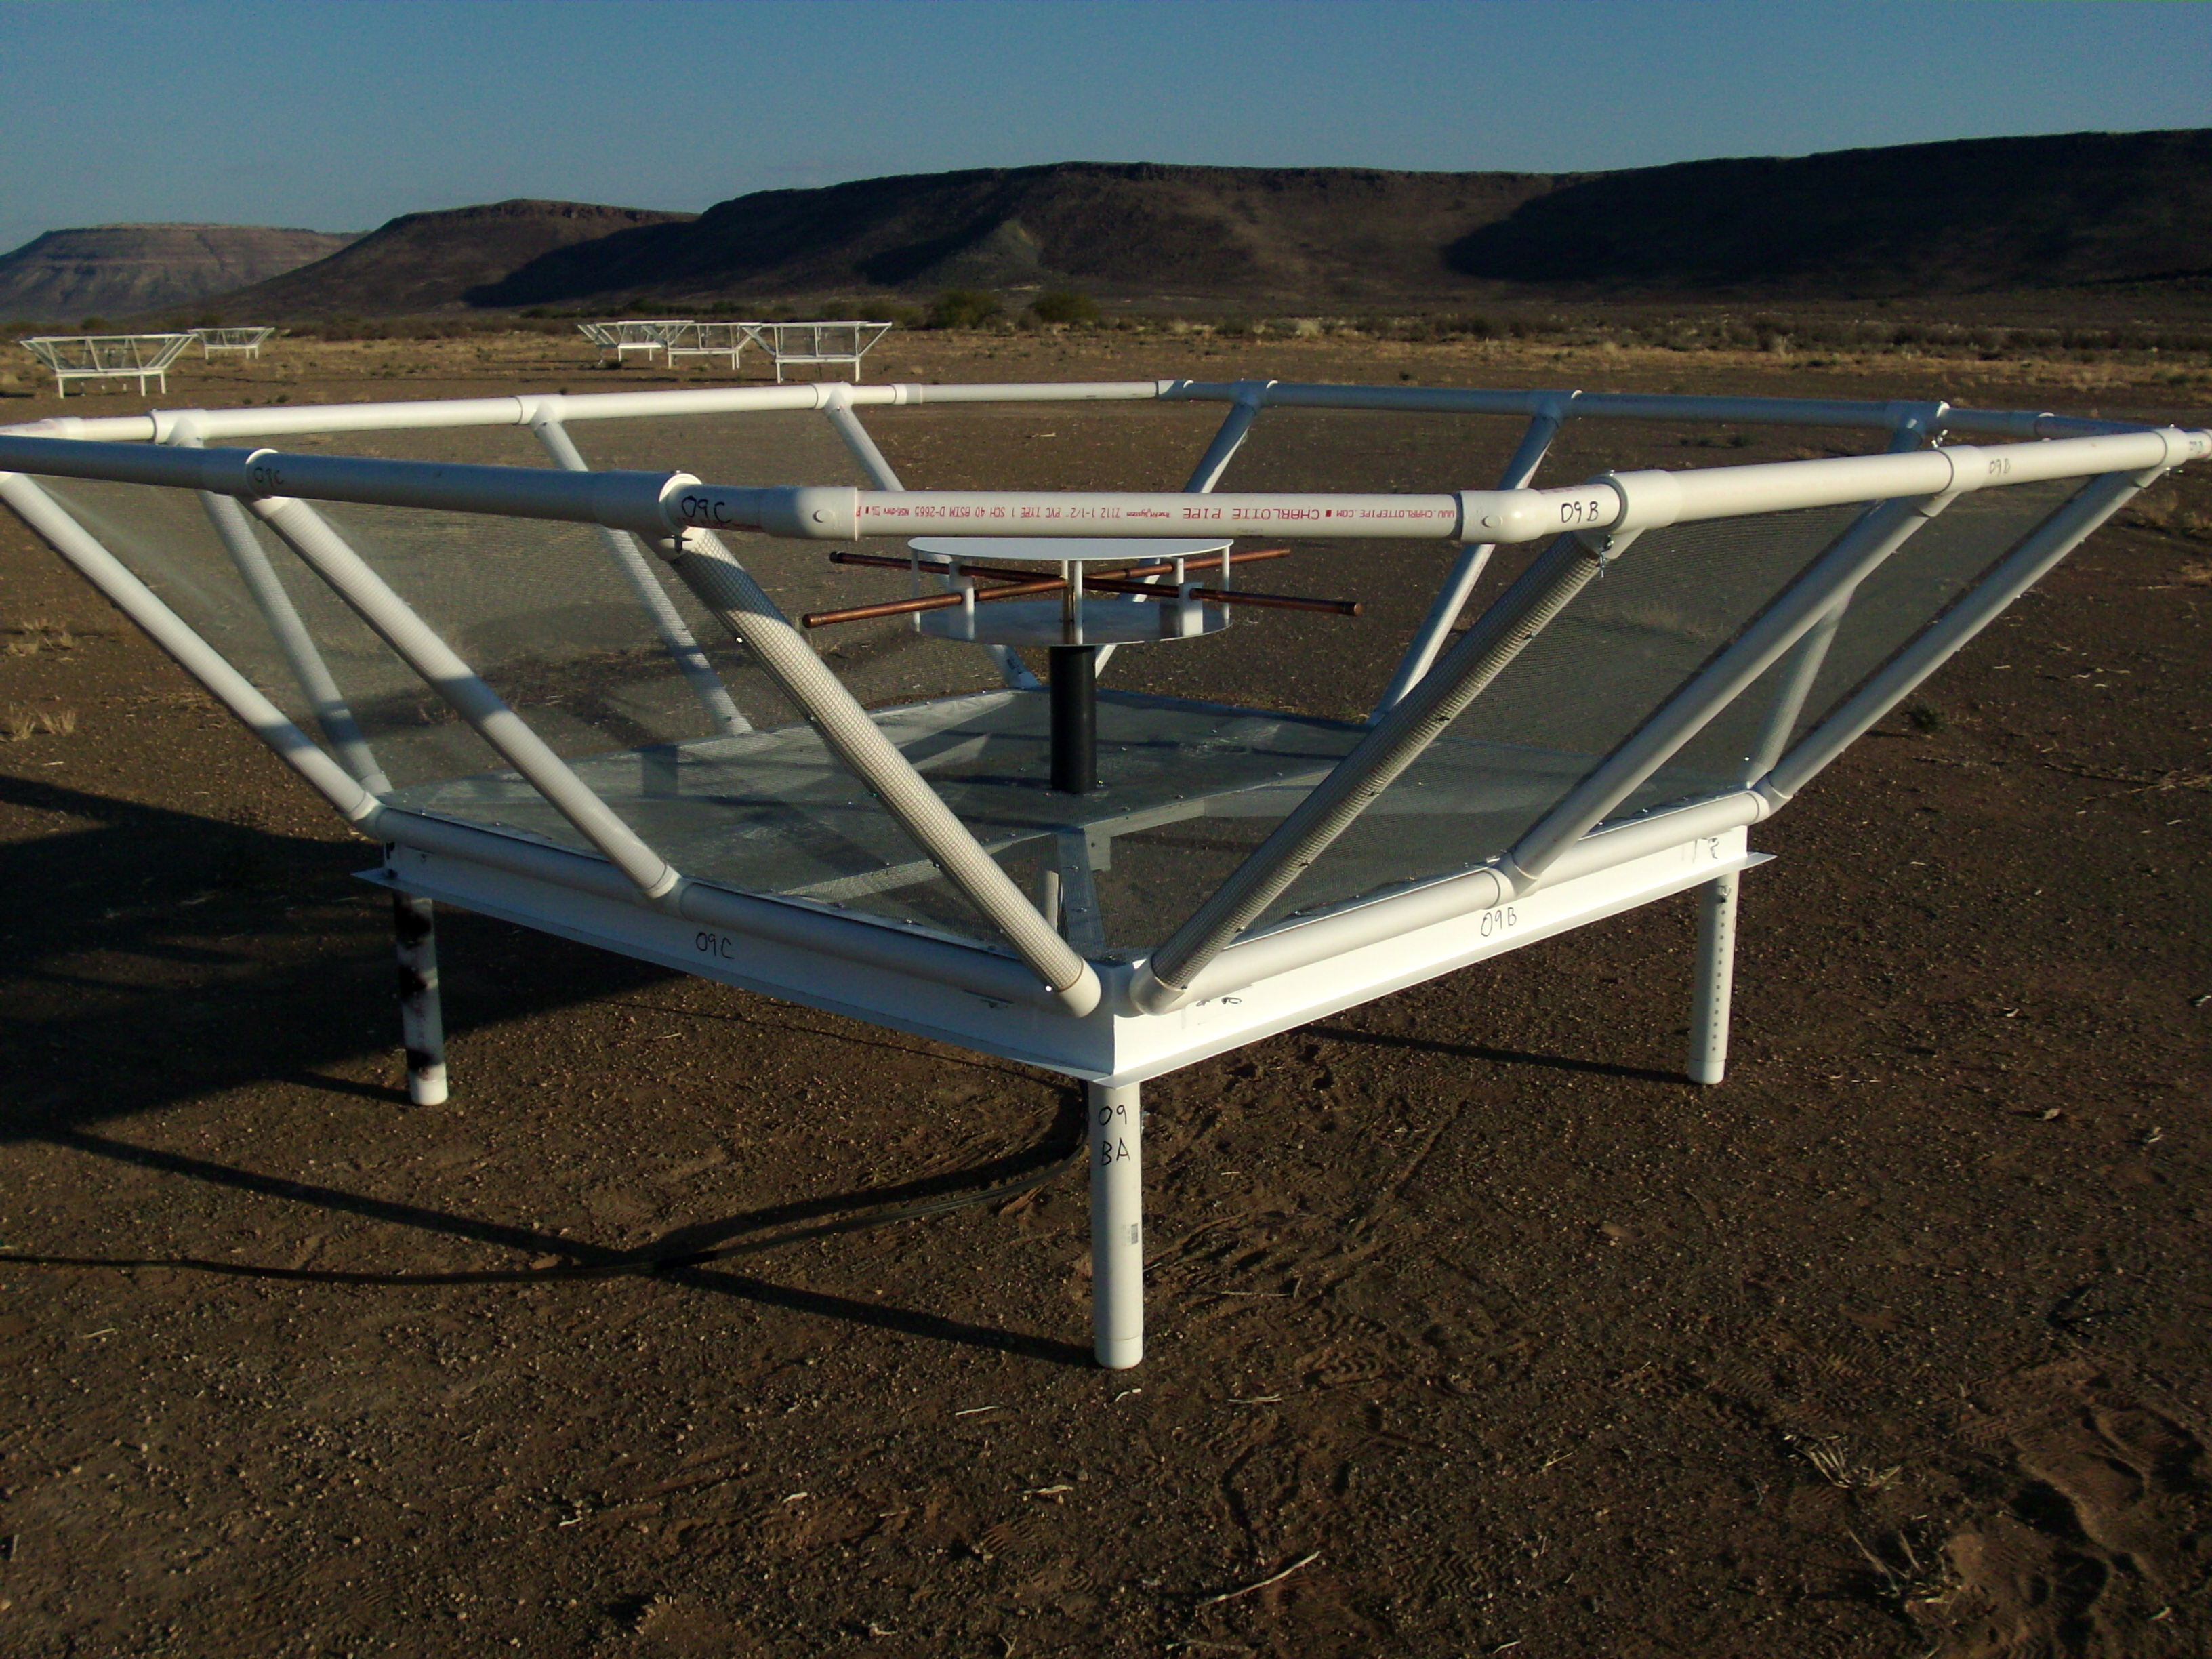
\includegraphics[height=0.35\textwidth]{plots/paper_dipole.png}
	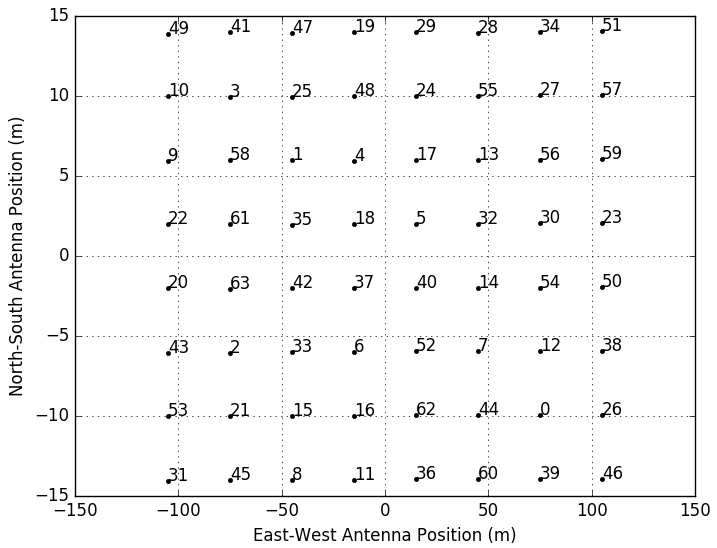
\includegraphics[height=0.35\textwidth]{plots/antenna_layout.png}
	\caption{PAPER dipole in South Africa (left) and PAPER-64 antenna layout (right).}
	\label{fig:paper}
\end{figure*}

PAPER-64 observed for a total of 135 nights between 2012-2013. The correlator processes a bandwidth of 100-200 MHz, corresponding to a redshift range of 6-12. For more information about the backend system of PAPER-64 and its observations, we refer the reader to \cc{??} and \citet{ali_et_al2015}.

Because there is a detailed discussion of the PAPER-64 data reduction pipeline in \citet{ali_et_al2015}, here we will only briefly summarize the data processing steps prior to the power spectrum analysis. 

Beginning with compressed data products which have been cleaned of radio frequency interference (RFI) at the $6\sigma$ level and then down-sampled (to $42.9$ s integrations, $203$ frequency channels), we then employ the technique of redundant calibration as a means of calibrating for individual antenna gains without needing to use information about the sky. Because PAPER is laid out on a grid, antenna calibration parameters can be found through the use redundancy. Namely, baselines of the same length and orientation should measure the same sky signal, but in practice there are differences due to instrumental effects caused by antennas, cables, and receivers. Using the basis of redundancy, however, allows us to set up a system of equations to solve for a complex gain per antenna that brings all baseline of a particular type into alignment. We perform these computations using the package OMNICAL \cc{citation needed}.

We next solve for the array's overall phase and gain calibration parameters using a standard self calibration method. We used radio sources Pictor A, Fornax A, and the Crab Nebula to fit for an overall phase solution, and set our overall flux scale using Pictor A as a calibrator source. Although PAPER-64 data exists for all $4$ polarizations, we only use the $xx$ and $yy$ polarization data to form Stokes I visibilities as $V_{I} = \frac{1}{2}(V_{XX} + V_{YY})$.

Eliminating bright foregrounds remains a challenging yet crucial component of any 21 cm data analysis. There are many techniques to go about foreground removal, including spectral polynomial fitting, principle component analysis, Fourier-mode filtering, non-parametric subtractions, and inverse covariance weighting. PAPER uses a delay-spectrum filtering method which was first explained and applied in \citet{parsons_et_al2014}. In short, the delay-filtering technique employs the spectrally smooth nature of foregrounds, which are consequently localized in delay-space, the Fourier dual to frequency. We subtract all components that fall within the horizon limit for a specific baseline type in delay-space, plus a $15$ ns buffer, thus gaining about $\sim4$ orders of magnitude in sensitivity. 

After removing an additional layer of RFI (values $3\sigma$ above the median), we average together all our data into two datasets: even julian dates and odd julian dates. A total of $124$ nights of data comprises this average.

Finally, our last analysis step before power spectrum estimation is the use of a fringe-rate filter. As shown in \citet{parsons_et_al2016}, a fringe-rate filter allows us to maximize our sensitivity even further by averaging visibilities in time. We apply this filter in the fringe-rate domain, the Fourier-dual to time, and it effectively amounts to increasing our data's integration time. Another way to describe the filter is that it weights different parts of the sky (which rotate at different ``fringe-rates") by the antenna beam. This allows us to up-weight parts of the sky high in the primary beam, and down-weight those that are less sensitive.

\begin{figure}
	\centering
	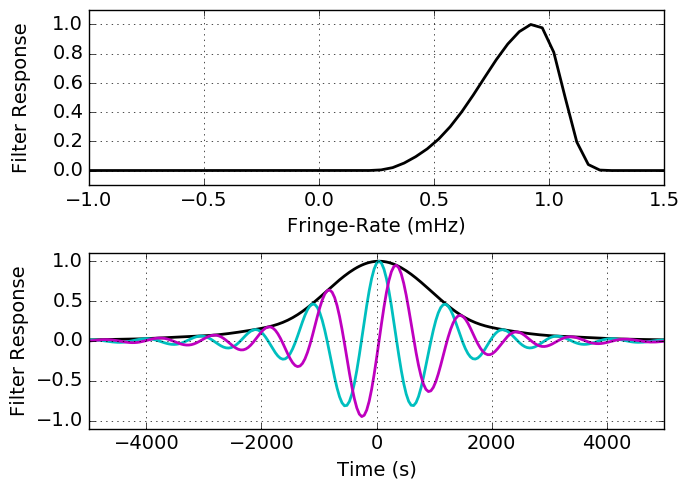
\includegraphics[width=\columnwidth]{plots/frp.png}
	\caption{The optimal fringe-rate filter used in the analysis, normalized to $1$.}
	\label{fig:frp}
\end{figure}

New to our updated PAPER-64 analysis is the use of an optimal fringe-rate filter, which maximizes our sensitivity. In \citet{ali_et_al2015}, the filter that was applied was degraded by widening it in fringe-rate space. This was chosen in order to decrease the resulting integration time, therefore increasing the number of independent modes and reducing signal loss associated with applying inverse covariance weighting on data with too few modes.

With the development of a robust method for assessing signal loss (see Section \ref{sec:Sigloss}), we feel comfortable using a narrow filter (Figure \ref{fig:frp}), which yields an effective integration time of $3857$ s (see Section \ref{sec:PSSense} for calculation) and $8$ total independent modes for our $8.5$ hours of LST. The filter is computed for a fiducial $30$ m baseline at $150$ MHz, the center frequency in our band. It is then implemented on a per baseline basis by convolving the time-domain visibilities with the Fourier transform of the fringe-rate filter, resulting in averaged visibilities yielding $\sim 2$ orders of magnitude in sensitivity. 

\subsection{Power Spectrum Estimation}
\label{sec:PS}

To form power spectrum quantities using our two fringe-rate filtered, LST-binned datasets, we use OQE methods as summarized in Section \ref{sec:SiglossOverview}. Here we will describe its application to PAPER-64 data. 

We have a $2$-dimensional data vector $\textbf{x}$ for each baseline and data group (`even' or `odd'). As part of our bootstrapping routine (and to speed things up), we divide up our total number of baselines into $5$ random, equal-sized groups (the way we bootstrap baselines into groups is explained in Section \ref{sec:Boot}). Taking $\textbf{x}$ to be the averaged data from all baselines within a group, we now have $10$ possible data vectors (for $5$ groups and $2$ datasets). 

Notice that there are two quantities of $\textbf{w}\textbf{x}$ in the expression for $\hat{\textbf{q}}$ in Equation \ref{eq:qhat}, representing two copies of weighted data. We perform all possible cross-multiplications of this quantity, except between the same datasets (`even' with `even', for example) and same groups (`baseline group 1' with `baseline group 1', for example). We avoid these computations to prevent the introduction of biases from shared auto power.

As mentioned previously, we have a choice for our normalization matrix $\textbf{M}$. For our analysis, we choose to compute it by taking the Cholesky decomposition of $\textbf{F}$. Namely, we decompose the Fisher matrix such that $\textbf{F} = \textbf{L}\textbf{L}^{\dagger}$, where $\textbf{L}$ is a lower triangular matrix. Next, we construct $\textbf{M} = \textbf{D}\textbf{L}^{-1}$, where \textbf{D} is a diagonal matrix. Hence, our window function $\textbf{W} = \textbf{MF}$ becomes $\textbf{W} = \textbf{D}\textbf{L}^{\dagger}$ and is an upper triangular matrix. This window function was constructed in a way to prevent the leakage of foreground power from low $k$ to high $k$ modes. Specifically, we order the elements in $\textbf{F}$ in such a way so that power can leak from high $k$ modes to low $k$ modes, but not vice versa. Since most foreground power shows up at low $k$'s, this method ensures a window function that retains clean, noise-dominated measurements.

In practice, our final power spectrum result is a $2$-dimensional quantity (a function of both time and $k$). We compute $20$ bootstraps of these quantities, where each bootstrap creates baseline groups randomly. We form both the quantity $\textbf{P(k)}$ and the folded version $\Delta^{2}\textbf{(k)}$, defined as:

\begin{equation}
\Delta^{\textbf{2}}\textbf{(k)} = \frac{k^{3}}{2\pi^{2}}\hat{\textbf{p}}\textbf{(k)}
\end{equation}

\section{Application: Signal Loss}
\label{sec:Sigloss}

As detailed in Section \ref{sec:SiglossOverview}, signal loss can arise from the interplay between fringe-rate filtering and inverse covariance weighting. In this section, we explain a methodology that simulates the injection and recovery of a cosmological signal in order to quantify the amount of signal loss. Before doing so however, we first explain how noise and EoR are created in our power spectrum pipeline, both of which are used to verify signal loss.

\subsection{Noise and EoR}

One critical new component of our power spectrum pipeline is that we have many different power spectrum channels that simultaneously get processed at the same time and are especially useful for computing signal loss and sensitivity estimations. Two important channels, in addition to our PAPER-64 data, are a noise dataset and an EoR dataset (in addition to these, we also look at different combinations of all three). We will briefly describe each.

We create random noise with a variance determined by the sensitivity of our instrument in order to best represent the thermal noise level of our data. We calculate our system temperature for our frequencies of interest as:

\begin{equation}
\label{eq:sys}
T_{sys} = 180\Big(\frac{\nu}{0.18}\Big)^{-2.55} + T_{rcvr}
\end{equation}

where $\nu$ are frequencies in GHz. We use a receiver temperature of $200$ K, yielding $T_{sys} = 487$ at $150$ MHz. This is lower than in \citet{ali_et_al2015} because \cc{why?}. We convert this temperature into a variance statistic using:

\begin{equation}
T_{rms} = \frac{T_{sys}}{\sqrt{\Delta\nu \Delta t N_{days} N_{pols}}}
\end{equation}

where $\Delta\nu$ is channel spacing, $\Delta t$ is integration time, $N_{days}$ is the number of data samples for a particular time and frequency that went into our LST binned set, and $N_{pols}$ is the number of polarizations ($2$ for Stokes I). Our simulated noise has the same shape as our data, and we fringe-rate filter it in the same way to best mimic the real noise floor of our data. 

A second additional important channel in our pipeline is a simulated EoR signal. We again simulate random noise (with a default scale of $1$) with the same shape as our data, and we fringe-rate filter this signal twice. The first filter transforms the unattached noise into a signal that's attached to the sky (i.e. what our instrument observes). The second filter represents the fringe-rate filtering step in our data analysis pipeline. This fake EoR signal is injected on top of data at various amplitude levels in order to measure its loss.

\subsection{Signal Loss Methodology} 

The loss of a cosmological signal when analyzing PAPER-64 data is a real and significant issue. To reiterate, when applying inverse covariance weighting, $\textbf{C}^{-1}$ is empirically estimated from the data itself, which has the consequence of over-fitting the noise in the data, producing power spectra values well below the thermal noise limit that is predicted based on observation parameters. This is especially prevalent when weighting fringe-rate-filtered data, which has so few independent time modes to begin with, leading to a noisier dataset. Being able to accurately quantify this loss is crucial in interpreting and providing credibility to any power spectrum limits. 

New to the PAPER-64 analysis is a robust method to estimate signal loss. This method is now a standard analysis step for all PAPER analyses and one that will be used for HERA moving forward.

As discussed previously, our power spectrum pipeline runs on a standardized set of channels (pure data, pure noise, pure EoR, and combinations of the three). As part of our signal loss routine, we also compute power spectra with various levels of the created EoR signal, dialing its amplitude from well-below the data level, to well-above. Suppose that $\textbf{e}$ is the injected EoR (at some amplitude level), and $\textbf{x}$ is our data vector. We define $\textbf{r}$ to be:

\begin{equation}
\textbf{r} = \textbf{x} + \textbf{e}
\end{equation}

Using OQE formalism, we are interested in the following two quantities: $P_{in}$ and $P_{out}$. The input power spectrum, $P_{in}$ represents the unweighted power spectrum of only $\textbf{e}$, our simulated EoR signal. The output power spectrum, $P_{out}$, is the weighted power spectrum of $\textbf{e}$ that would result from our pipeline if the signal was mixed with our data. Comparing the two quantities yields insight into how much of $\textbf{e}$ is lost due to our choice of weighting. Ignoring normalization, factors:

\begin{equation}
P_{in} \propto \textbf{e}^{\dagger}\textbf{I}\textbf{Q}\textbf{I}\textbf{e}
\end{equation}

\begin{eqnarray}
\label{eq:sigloss}
P_{out} \equiv \textbf{P}_{e} &=& \textbf{P}_{r}-\textbf{P}_{x} \nonumber \\
&\propto& \textbf{r}^{\dagger}\textbf{w}_{r}\textbf{Q}\textbf{w}_{r}\textbf{r} - \textbf{x}^{\dagger}\textbf{w}_{x}\textbf{Q}\textbf{w}_{x}\textbf{x} 
\end{eqnarray}

It is noted that the output power spectrum is comprised of two terms: the power spectrum associated with \textbf{r}, and that of data \textbf{x} alone. 

One may wonder why $P_{out}$ cannot be computed simply as the weighted power spectrum of $\textbf{e}$ alone, namely $P_{out} \propto \textbf{e}^{\dagger}\textbf{w}_{e}\textbf{Q}\textbf{w}_{e}\textbf{e}$. Expanding Equation \ref{eq:sigloss}:

\begin{eqnarray}
P_{out} &\propto& (\textbf{x}+\textbf{e})^{\dagger}\textbf{w}_{r}\textbf{Q}\textbf{w}_{r}(\textbf{x}+\textbf{e}) - \textbf{x}^{\dagger}\textbf{w}_{x}\textbf{Q}\textbf{w}_{x}\textbf{x} \nonumber \\
&\propto& \textbf{x}^{\dagger}\textbf{w}_{r}\textbf{Q}\textbf{w}_{r}\textbf{x} + \textbf{e}^{\dagger}\textbf{w}_{r}\textbf{Q}\textbf{w}_{r}\textbf{e} + \textbf{x}^{\dagger}\textbf{w}_{r}\textbf{Q}\textbf{w}_{r}\textbf{e} \nonumber \\
&+& \textbf{e}^{\dagger}\textbf{w}_{r}\textbf{Q}\textbf{w}_{r}\textbf{x} - \textbf{x}^{\dagger}\textbf{w}_{x}\textbf{Q}\textbf{w}_{x}\textbf{x} \nonumber 
\end{eqnarray}

And taking the case of very large $\textbf{e}$, so that $\textbf{w}_{r} \sim \textbf{w}_{e}$ and any terms involving only $\textbf{x}$ are small:

\begin{eqnarray}
P_{out, \textbf{e} \gg \textbf{x}} &\propto& \textbf{e}^{\dagger}\textbf{w}_{e}\textbf{Q}\textbf{w}_{e}\textbf{e} + \textbf{x}^{\dagger}\textbf{w}_{e}\textbf{Q}\textbf{w}_{e}\textbf{e} \nonumber \\
&+& \textbf{e}^{\dagger}\textbf{w}_{e}\textbf{Q}\textbf{w}_{e}\textbf{x}
\end{eqnarray}

We see that our naive expression for $P_{out}$ is the first term, but there also two additional terms. An initial assumption would be that the cross-terms that involve both $\textbf{e}$ and $\textbf{x}$ should be zero, since the two quantities are un-correlated. However, \cc{need explanation about power in cross-terms here}. Therefore, in our investigation of signal loss, we use the full quantity for $P_{out}$ as in Equation \ref{eq:sigloss}.

For the unweighted case ($\textbf{w} \equiv \textbf{I}$), we expect $P_{out}$ and $P_{in}$ to be equal, and hence the ratio of $P_{in} / P_{out}$ to be 1. For the weighted case, this is not true due to signal loss. In order to quantify the loss, we look at the ratio of $P_{in}$ to $P_{out}$ as the amplitude level of the injected signal \textbf{e} is increased. In the next section, we highlight two methods that yield similar results for the determination of signal loss using $P_{in}$ and $P_{out}$

\subsection{Signal Loss in Practice}

We now shift our attention towards computing signal loss for fringe-rate filtered PAPER-64 dataset, using inverse covariance weighting ($\textbf{w} = \textbf{C}^{-1}$). Our expressions for $P_{in}$ and $P_{out}$ become:

\begin{eqnarray}
P_{in} &\propto& \textbf{e}^{\dagger}\textbf{I}\textbf{Q}\textbf{I}\textbf{e} \\
P_{out} &\propto& \textbf{r}^{\dagger}\textbf{C}_{r}^{-1}\textbf{Q}\textbf{C}_{r}^{-1}\textbf{r} - \textbf{x}^{\dagger}\textbf{C}_{x}^{-1}\textbf{Q}\textbf{C}_{x}^{-1}\textbf{x} 
\end{eqnarray}

Using the input and output power spectra for range of EoR amplitudes, we use two methods to determine signal loss associated with the over-fitting of noise during inverse covariance weighting. 

\cc{Determine whether we want to show pure noise plots, or just data, or both!!!}

The first method is very straightforward. Post-bootstrapping, our final power spectra are 1-dimensional and only a function of $k$. For each $k$, we simply look at $P_{out}$ as a function of $P_{in}$, as shown in Figure \ref{fig:sigloss1_noise}. The shape of this function can be explained as follows. At small injection levels (small $\textbf{e}$), $P_{out}$ and $P_{in}$ are equal, and there is no signal loss. As the amplitude of EoR increases, we then move into a regime where the final output power spectrum is lower than the unweighted input one. This is dangerous, because without correcting for this effect one might be led to underestimate the EoR signal. The peculiar tail at very low injection levels (where $P_{out} > P_{in}$) is an unphysical feature, but rather illustrates that there is some non-negligible cross-term power between $\textbf{n}$ and $\textbf{e}$.

For this method, we interpolate the signal loss factor (per $k$), computed as $P_{in}/P_{out}$, at a $P_{out}$ value equal to the $2\sigma$ power spectrum upper limit of noise alone. In other words, we look at $P_{noise} \propto \textbf{n}^{\dagger}\textbf{C}_{n}^{-1}\textbf{Q}\textbf{C}_{n}^{-1}\textbf{n}$, compute its $2\sigma$ upper limit (mean over bootstraps + $2 \times $standard deviation over bootstraps), and interpolate the value of $P_{in}/P_{out}$ at this value. We therefore end up with one signal loss correction factor per $k$. 

\begin{figure*}
	\centering
	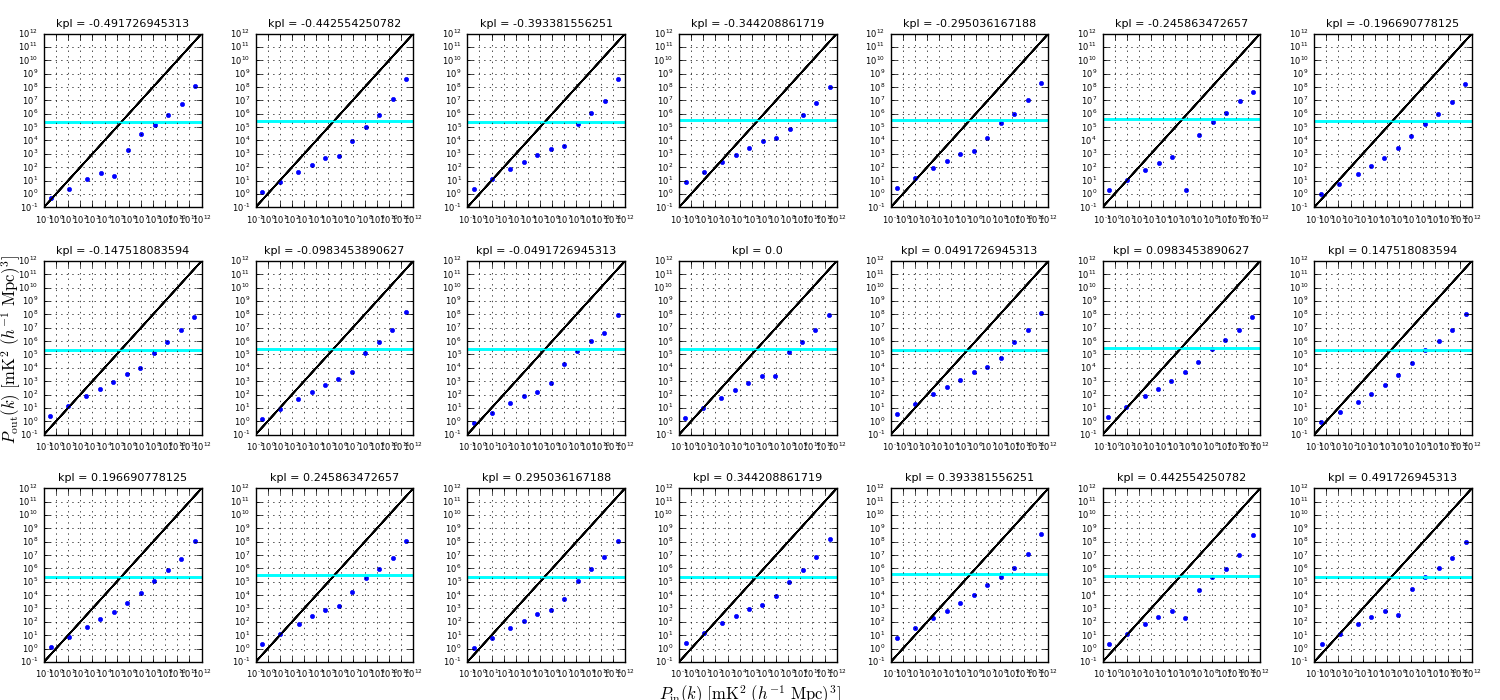
\includegraphics[width=1.0\textwidth]{plots/sigloss1_noise.png}
	\caption{$P_{in}$ vs. $P_{out}$ (blue points) for 15 injection levels and 21 $k$'s. The solid cyan line is the $2\sigma$ upper limit for the weighted power spectrum of noise alone, and it is at this level where the signal loss factor $P_{in}/P_{out}$ is computed by interpolation. \cc{Maybe re-do this plot with closer-together points}}
	\label{fig:sigloss1_noise}
\end{figure*}

Figure \ref{fig:ps1_noise} shows the power spectrum of our noise simulation, using full inverse covariance weighting, both before and after signal loss correction. Prior to signal loss correction, it is obvious that the power spectrum is unfeasible because it is well below the theoretical noise level prediction. Post-correction, the power spectrum values blow up much higher than both the theory and unweighted power spectrum. This is an effect caused by the steep nature of the eigenspectrum of $\textbf{C}$, and is explained more in Section \ref{sec:Weight}.

\cc{Need a plot that shows our signal loss factors are CORRECT. How to do that??}

\begin{figure*}
	\centering
	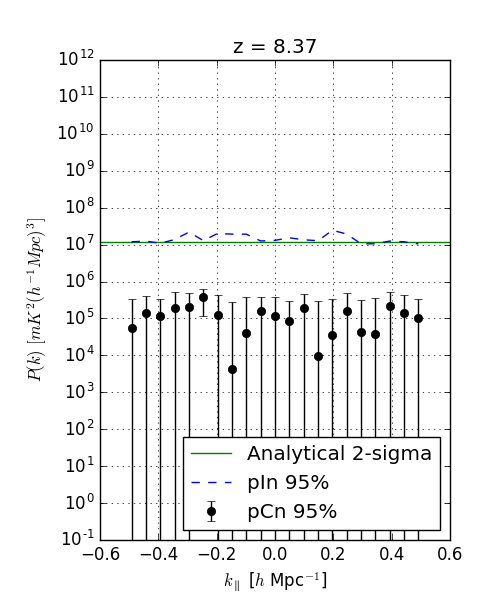
\includegraphics[width=0.4\textwidth]{plots/ps1_noise_nosigloss.png}
	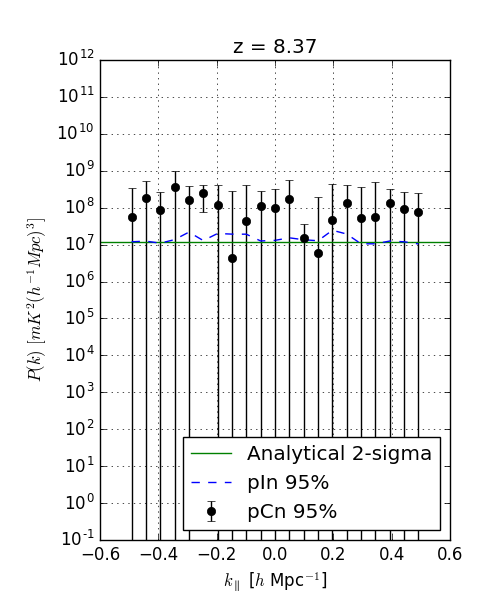
\includegraphics[width=0.4\textwidth]{plots/ps1_noise.png}
	\caption{Full inverse covariance weighted power spectrum of pure noise (black points, with $2\sigma$ error bars) before signal loss correction (left) and after (right). The dashed blue line is the unweighted power spectrum ($2\sigma$ upper limit). The solid green line is the theoretical noise level prediction based on observational parameters. \cc{Color negative points grey}}
	\label{fig:ps1_noise}
\end{figure*}

Our second method for estimating signal loss is similar to the first, but more comprehensive in a statistical sense. Instead of looking at input and output power spectra after bootstrapping, we now look at their values for every bootstrap in order to get a sense of their distributions. Figure \ref{fig:sigloss2_noise} plots $P_{in}$ vs. $P_{out}$ for $20$ bootstraps, and as expected, the function now has a spread in the width-direction in comparison to what was plotted in Figure \ref{fig:sigloss1_noise}, but otherwise shows a familiar trend. Similarly, our weighted noise power spectra also has a defined spread due to bootstrapping.

Using these two distributions ($P_{in}/P_{out}$ and $P_{noise}$), we can create bins along the $P_{noise}$ axis to yield histograms of signal loss factors for each bin. We similarly sort the values of $P_{noise}$ into the same bins, and multiply the probability of $P_{noise}$ per bin (the number of values falling into that bin, divided by the total) with the signal loss factors in that bin, essentially computing a weighted average across all bins to obtain a final signal loss factor per $k$. As shown in Figure \ref{fig:ps2_noise}, the results are very similar to the previous method. For future power spectrum results, we choose to use the second method because it computes final signal loss values using our full distributions of measurements.

One thing to note is that for both methods, we have been careful to validate that the computations yield no signal loss (signal loss factors of $1$) for the unweighted power spectrum case, as is expected. This is important in confirming that signal loss is a direct result of the choice for $\textbf{C}$.

\begin{figure*}
	\centering
	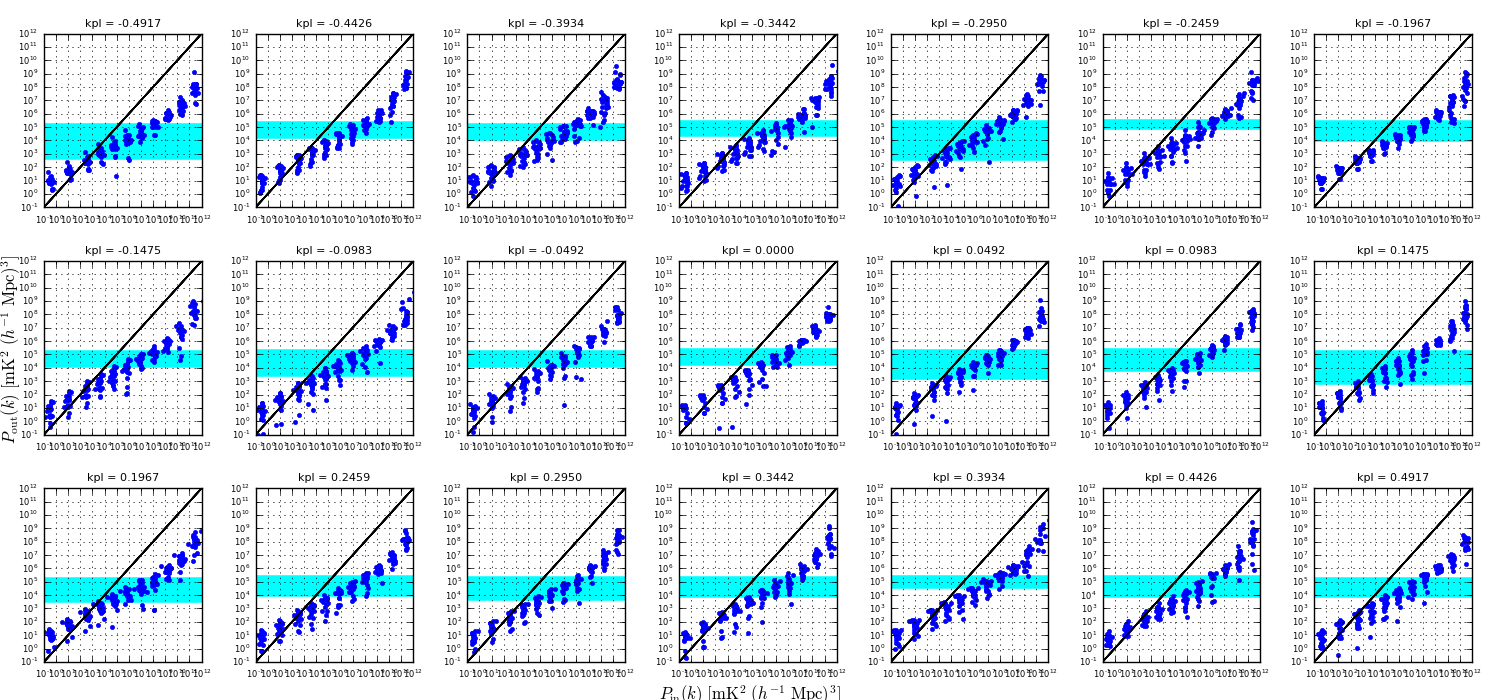
\includegraphics[width=1.0\textwidth]{plots/sigloss2_noise.png}
	\caption{$P_{in}$ vs. $P_{out}$ (blue) for 15 injection levels, 20 bootstraps, and 21 $k$'s. \cc{Plot a semi-transparent cyan range of pCn values instead of just the max}}
	\label{fig:sigloss2_noise}
\end{figure*}

\begin{figure*}
	\centering
	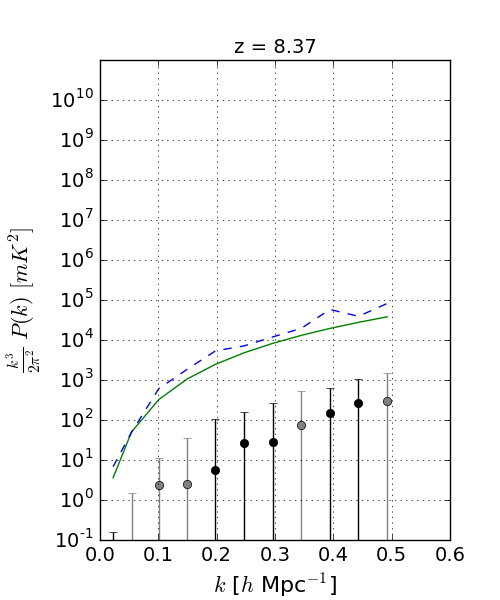
\includegraphics[width=0.4\textwidth]{plots/ps2_noise_nosigloss.png}
	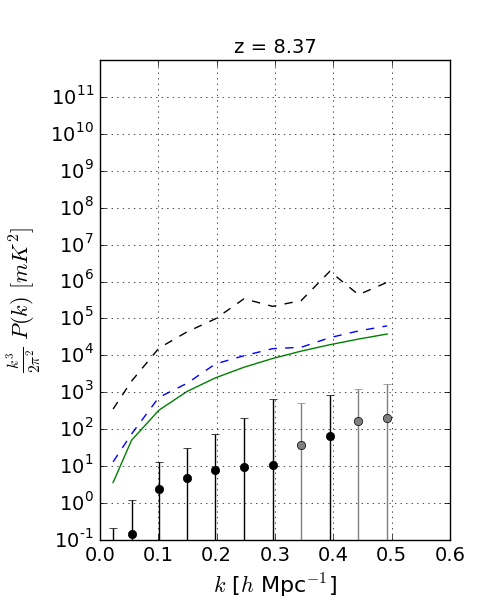
\includegraphics[width=0.4\textwidth]{plots/ps2_noise.png}
	\caption{Full inverse covariance weighted power spectrum of pure noise (black and grey points, with $2\sigma$ error bars) before signal loss correction (left) and after (right). Black points correspond to positive values, while grey points correspond to originally negative values that have been made positive for plotting. The dashed blue line is the unweighted power spectrum ($2\sigma$ upper limit). The solid green line is the theoretical noise level prediction based on observational parameters.}
	\label{fig:ps2_noise}
\end{figure*}

\subsection{Data Weighting}
\label{sec:Weight}

With our signal loss formalism established, we now have the capability of experimenting with different weighting options for $\textbf{w}$. Our goal here is to choose a weighting method that successfully down-weights foregrounds and systematics in our data without generating large amounts of signal loss. We have found that the balance between the two is a delicate one and requires a careful understanding and altering of covariance matrices.

We now turn our attention to power spectra using the 30 m East/West baselines of PAPER-64. Our dataset spans $8.5$ hours of LST ($.1$-$8.6$ hrs), includes a total of $51$ baselines, and is fringe-rate filtered using an optimal fringe-rate filter. We have two datasets (even days and odd days), and only cross-multiply data from different days and different baselines. We are interested in $21$ frequency channels (channels 95-115), which yields a power spectrum for a redshift of $z=8.4$. 

Using full inverse covariance weighting, our results are not too dissimilar to that of pure noise. Signal loss factors (Figure \ref{fig:sigloss2_data}) are of similar order of magnitude, and our power spectrum blows up past the unweighted version after signal loss correction (Figure \ref{fig:ps2_data}).

%\begin{figure*}
%	\centering
%	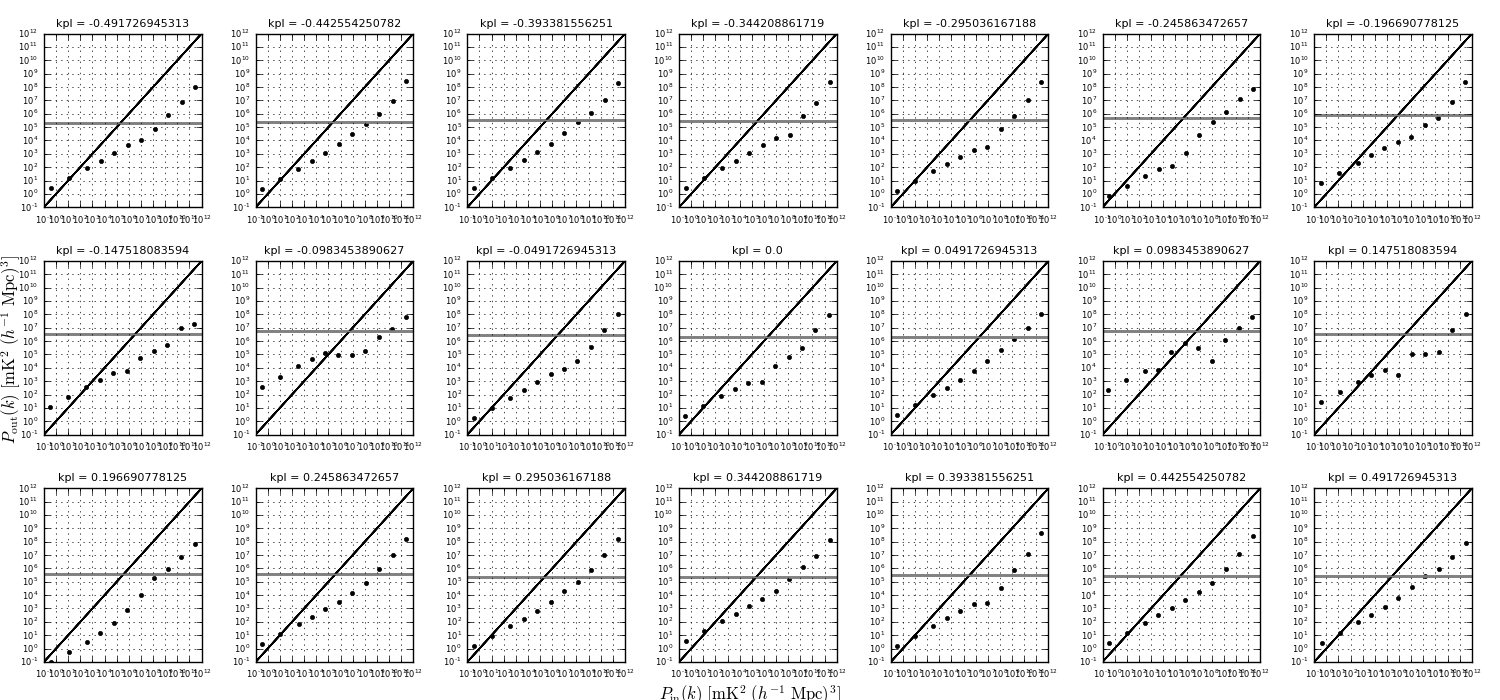
\includegraphics[width=1.0\textwidth]{plots/sigloss1_data.png}
%	\caption{$P_{in}$ vs. $P_{out}$ (black) for 15 injection levels and 21 $k$'s. The solid grey line is the $2\sigma$ upper limit for the weighted power spectrum of data alone, and it is at this level where the signal loss factor $P_{in}/P_{out}$ is computed by interpolation. \cc{Probably don't need to show this plot at all}}
%	\label{fig:sigloss1_data}
%\end{figure*}

\begin{figure*}
	\centering
	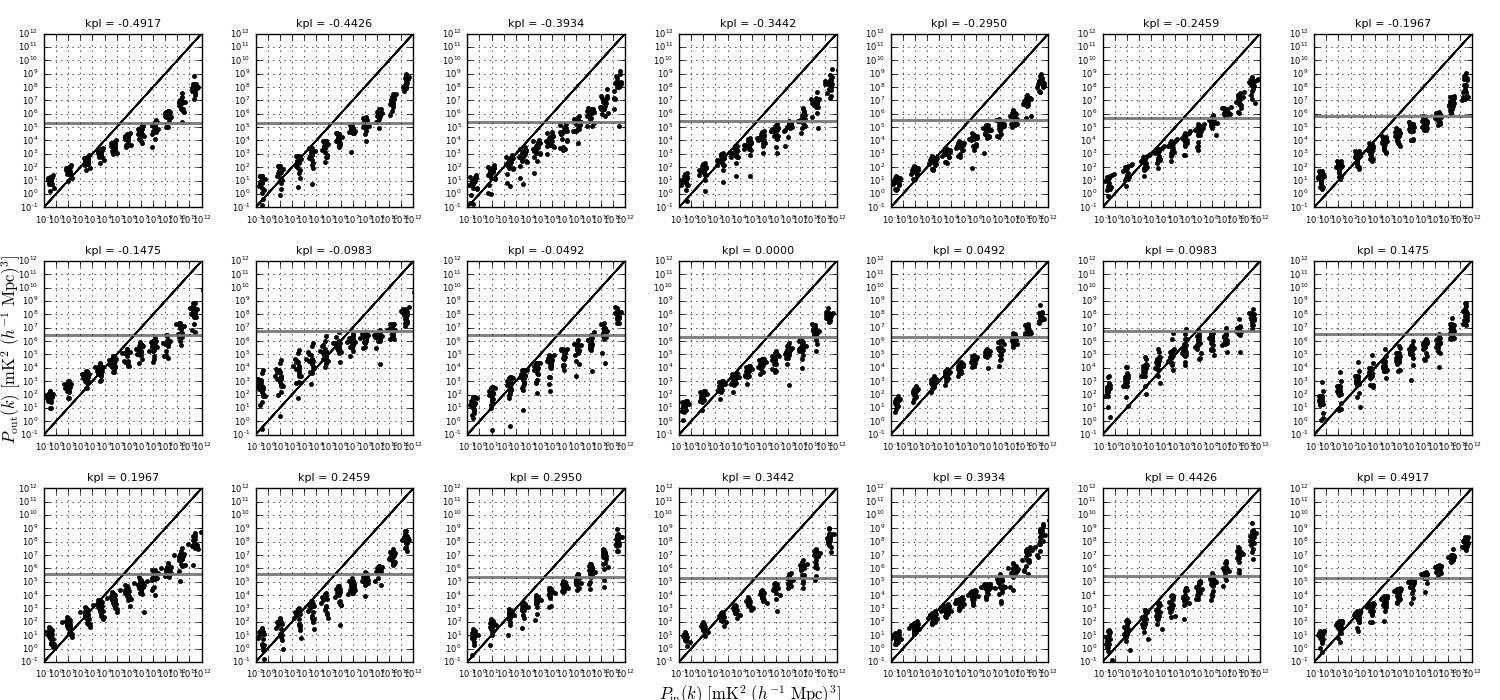
\includegraphics[width=1.0\textwidth]{plots/sigloss2_data.png}
	\caption{$P_{in}$ vs. $P_{out}$ (black) for 15 injection levels, 20 bootstraps, and 21 $k$'s. \cc{Plot a semi-transparent grey range of pCv values instead of just the max}}
	\label{fig:sigloss2_data}
\end{figure*}

\begin{figure*}
	\centering
	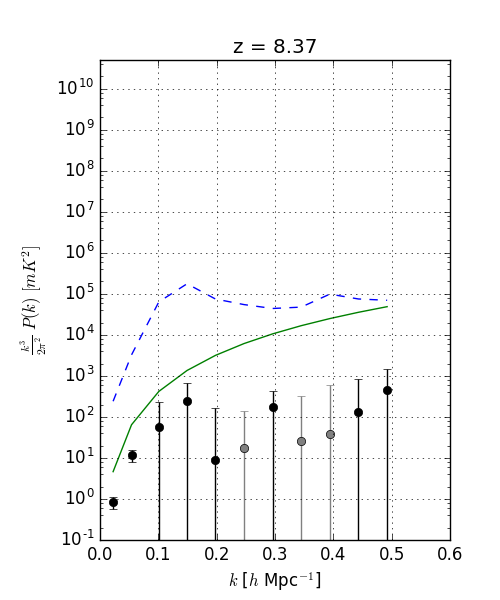
\includegraphics[width=0.4\textwidth]{plots/ps2_data_nosigloss.png}
	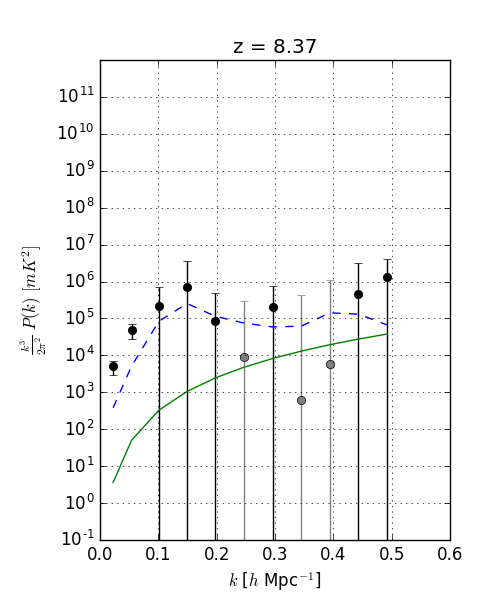
\includegraphics[width=0.4\textwidth]{plots/ps2_data.png}
	\caption{Full inverse covariance weighted power spectrum of PAPER-64 data (black and grey points, with $2\sigma$ error bars) before signal loss correction (left) and after (right). Black points correspond to positive values, while grey points correspond to originally negative values that have been made positive for plotting. The dashed blue line is the unweighted power spectrum ($2\sigma$ upper limit). The solid green line is the theoretical noise level prediction based on observational parameters.}
	\label{fig:ps2_data}
\end{figure*}

Looking into this behavior in more detail, we investigate the shape of the eigenspectrum of $\textbf{C}$ for a typical baseline used in the analysis. Figure \ref{fig:eigenspectrum} shows this spectrum for baseline (1,4). Most obviously, the spectrum is steep, spanning 4 orders of magnitude. Not as obvious is the effect of this shape on our results. When the matrix $\textbf{C}$ is inverted to form $\textbf{C}^{-1}$, the effect of the steepness of the eigenspectrum is to up-weight very few modes of the sky while the rest are drastically down-weighted. More specifically, our fringe-rate filtered data contains a finite, small number of independent modes, thereby resulting in a covariance matrix that can be described by just a few modes. Beyond the first few modes, the eigenvalues of each additional mode falls of dramatically. When inverting, we end up not only down-weighting those initial modes but severely up-weighting a few insignificant ones. Because of our weighting choice, signal loss blows up as it thinks we only have a couple modes in our data.

\begin{figure*}
	\centering
	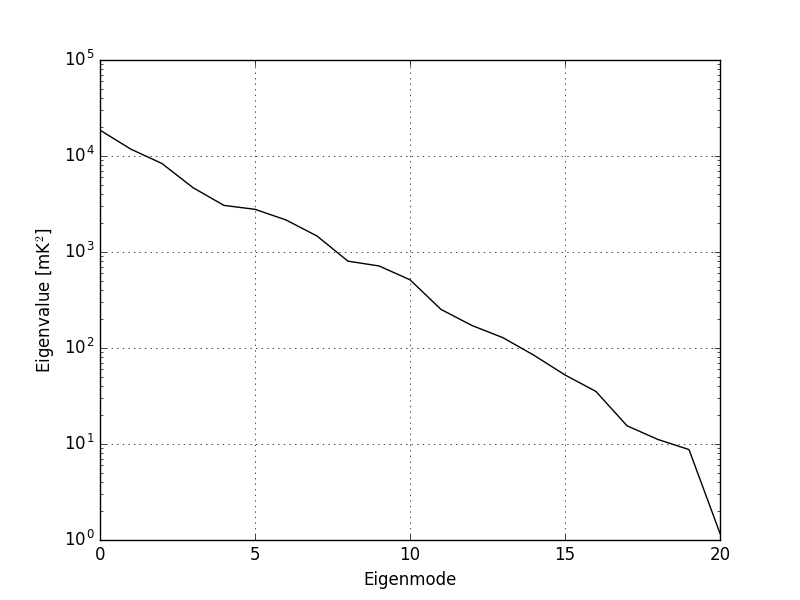
\includegraphics[width=0.4\textwidth]{plots/eigenspectrum.png}
	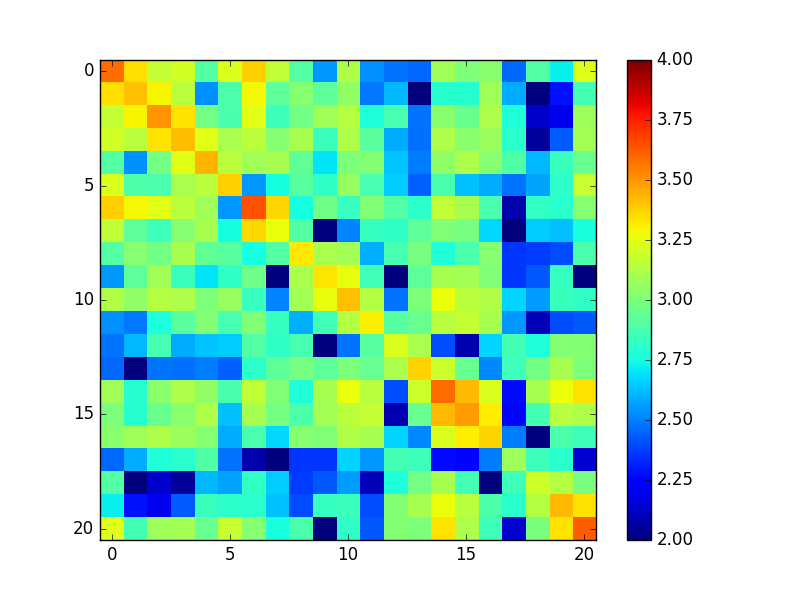
\includegraphics[width=0.4\textwidth]{plots/covariance.png}
	\caption{Eigenspectrum for $\textbf{C}$ for baseline (1,4) for the 21 channels ofs interest (left) and covariance matrix $\textbf{C}$ for the same baseline (right).}
	\label{fig:eigenspectrum}
\end{figure*}

Clearly the full inverse covariance treatment of our data is suboptimal to even the unweighted case, but we would like to find a weighting method that does successfully down-weight contaminants in our data and make some improvement over the unweighted power spectrum. There are many choices for determining the covariance matrix $\textbf{C}$, but here we will illustrate \cc{?} promising ones as applied to PAPER-64.

\cc{TO DO: decide on/explain/show different weightings}

\section{Application: Error Estimation}
\label{sec:Error}

\subsection{Thermal Noise}
\label{sec:PSSense}

One way to estimate errors of a $21$ cm power spectrum estimate is to compute theoretical errors based on instrumental temperature and observational parameters. A theoretical noise limit provides a useful cross-check for bootstrapped errors and is a helpful predictor of the maximum sensitivity that can achieved by a particular observation and analysis. Here we walk through a detailed computation of a theoretical noise estimation as applied to PAPER-64 observations and highlight major changes from \citet{ali_et_al2015}. We first give a general formula, and then go into detail about each factor.

The sensitivity prediction for a power spectral analysis of interferometric $21$ cm data, in temperature-units, is:

\begin{equation}
p(k) = \frac{X^{2}Y \Omega_{eff} T_{sys}^{2}}{\sqrt{2N_{lsts}N_{seps}}\,t_{int}N_{days}N_{bls}N_{pols}}
\end{equation}

\begin{itemize}
\item $X^{2}Y$: Conversion factors from observing coordinates (angles on the sky) to cosmological coordinates (co-moving distances). For $z=8.4$, $X^{2}Y = 5 \times 10^{11} [h^{-3} Mpc^{3} / str \, GHz]$.
\item $\Omega_{eff}$: The primary beam angular size. The effective beam area changes with the application of a fringe-rate filter, since parts of the beam are up-weighted and down-weighted. Using numbers from Table 1 in \citet{parsons_et_al2016}, $\Omega_{eff} = 0.74^{2}/0.24$ for an optimal fringe-rate filter. 
\item $T_{sys}$: The system temperature is set by Equation \ref{eq:sys}, for a receiver temperature of $200$ K and center frequency of $0.15$ GHz. 
\item $\sqrt{2}$: This factor in the denominator of the sensitivity equation comes from only using the real part of power spectrum estimates when plotting and quoting upper limits.
\item $N_{lsts}$: The number of LST hours that go into power spectrum estimation. The sensitivity scales as the square root because we integrate incoherently over time. For PAPER-64, $N_{lsts} = 8$ hours.
\item $N_{seps}$: The number of baseline separation types averaged incoherently in a final power spectrum estimate. For the analysis in this paper, we only use one type of baseline, hence $N_{seps}=1$.
\item $t_{int}$: The integration time of the data. It is crucial to adapt this number if filtering is applied along the time axis (i.e. a fringe-rate filter). We compute the effective integration time of our fringe-rate filtered data by... For PAPER-64, this number is $t_{int} = 3857$ s. 
\item $N_{days}$: The total number of days of data analyzed. 
\item $N_{bls}$:
\item $N_{pols}$: The number of polarizations averaged together. For the case of Stokes I, $N_{pols}=2$.
\end{itemize}

\subsection{Bootstrapping}
\label{sec:Boot}

In this section, we highlight two major changes since \citet{ali_et_al2015}, using the lessons we've learned about sampling with replacement and bootstrapping independent samples.
\cc{Include info about baseline bootstrapping:}
For the \citet{ali_et_al2015} method, each group is then sampled with replacement to create a new group, of the same size, that can have repeated baselines inside it. We discover that in doing so, we are sacrificing some of our sensitivity since this results in there being 3-4 repeated baselines per group. In order to maximize our sensitivity but still apply random sampling for use in error estimation, we instead form new groups using all independent baselines except the very last one. For example, if we have $10$ baselines in a group, we use the first $9$ to guarantee at least $9$ independent measurements, and then fill the last slot randomly out of the $10$. We do this for all $5$ groups. This is still a valid means of bootstrapping because there are many more possibilities of baseline groupings than the number of bootstraps we run for this analysis ($nboots = 20$).

\cc{Include info about second round of bootstrapping:}
In \citet{ali_et_al2015}, a second round of bootstrapping occurs over the bootstrap and time axes simultaneously. Random values are sampled with replacement along both axes, drawing as many values as there are number of bootstraps and times. Final power spectrum limits are then computed by taking the mean and standard deviation over this second bootstrap axis. 

However, we have found that this method greatly underestimates power spectrum errors, especially for fringe-rate filtered data. This can be explained by the fact that fringe-rate filtered data has a dramatically reduced number of independent modes. Hence, drawing $100$ samples out of a length-$100$ dataset that only has $5$ independent modes in it, for example, results in a narrower distribution of values that leads to a false error estimation.

To avoid this issue, we instead take a simple average along the time axis. Our final power spectrum limits are computed by taking the mean and standard deviation over our single bootstrap axis. 


\section{Application: Bias}
\label{sec:Bias}


\section{Conclusion}
\label{sec:Con}

\section{Acknowledgements}
\cc{NSF Graduate Research Fellowship Program (GRFP) Fellowship}
\cc{UC Berkeley Chancellor's Fellowship}
\label{sec:Ack}

\bibliographystyle{apj}
\bibliography{refs}


\end{document}

